\part{Experiments and Validation}

In this part we present some of the results we obtained with our system on several experiments.

In order to evaluate our system, we experimented on three kinds of test cases. We started with small, \enquote{academic}, test cases, which were used to evaluate and tune the cooperative behavior of the agents. The optimization performances of the systems were then tested on bigger, \enquote{real-world} test cases [[and in some cases compared with existing methods]]. At last, we produced a third type of test cases which are automatically generated, in order to test raw performances and scalability properties of our system.

We also made additional experiments in order to evaluate others functionalities of our systems: uncertainties propagation and adaptations to changes.

\chapter{Academic Test Cases}

[[TODO: introduce better the different test cases]]

[[need an overhaul of the section]]

In this section we present several test cases: Alexandrov Problem, Turbofan Problem, Viennet1 and Rosenbrock valley, on which our system has been applied, and the experimental results we obtained. In each test cases, the MAS consistently converges towards the best (or one of the best) solution.

\begin{figure}
\centering
	\begin{subfigure}[b]{0.4\textwidth}
		$\begin{array}{c}
			a_1 = (l_1 - a_2)/2 \\
			a_2 = (l_2 - a_1)/2 \\
			min \; \frac{1}{2}(a_1^2 + 10a_2^2 + 5(s-3)^2) \\
			subject \; to \\
			s + l_1 \leq 1 \\
			-s + l_2 \leq -2
		\end{array}$
		\caption{mathematical formulation.}\label{alexandrov:math}
	\end{subfigure}
	\hfill%for spacing
	\begin{subfigure}[b]{0.5\textwidth}
		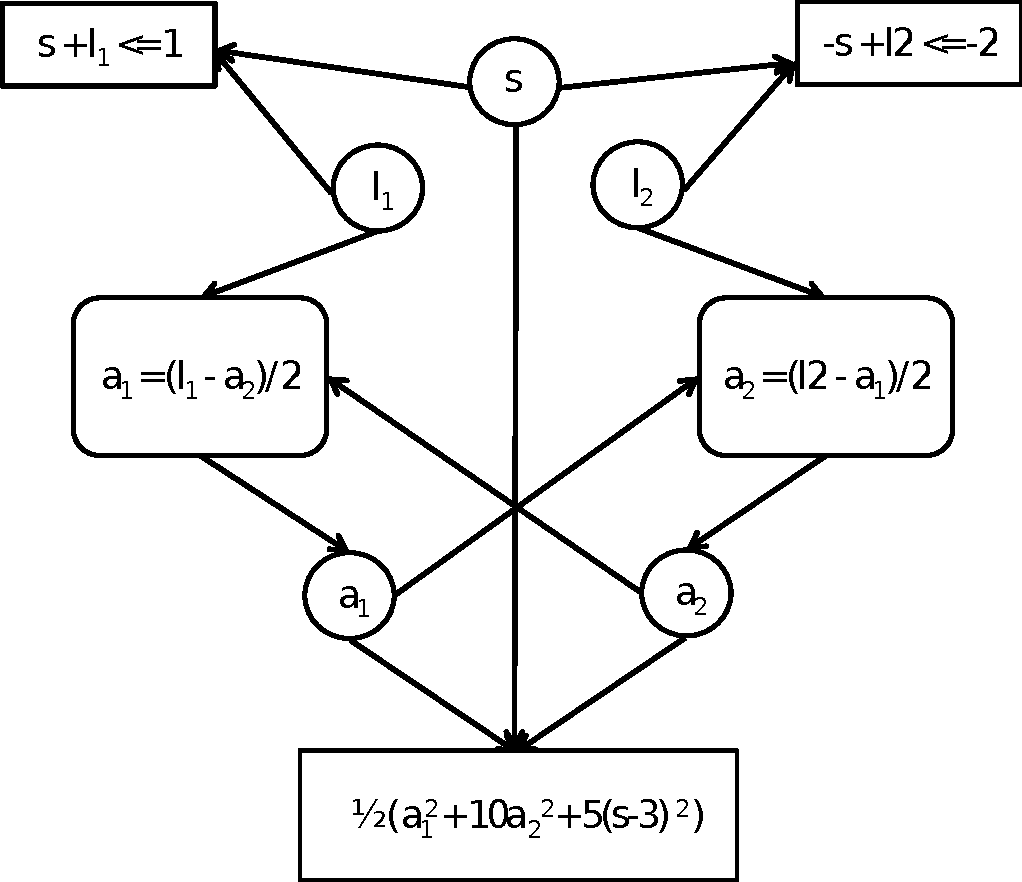
\includegraphics[width=\textwidth]{testcases-Alexandrov}%screen_Alexandrov}%}
		\caption{corresponding agent graph.}\label{alexandrov:graph}
	\end{subfigure}
\caption{Alexandrov problem}\label{alexandrov}
%\vspace{-20pt}
\end{figure}

\section{Alexandrov Problem}

\begin{figure}[]
\centering
  	\begin{subfigure}[b]{0.4\textwidth}
		\centering
		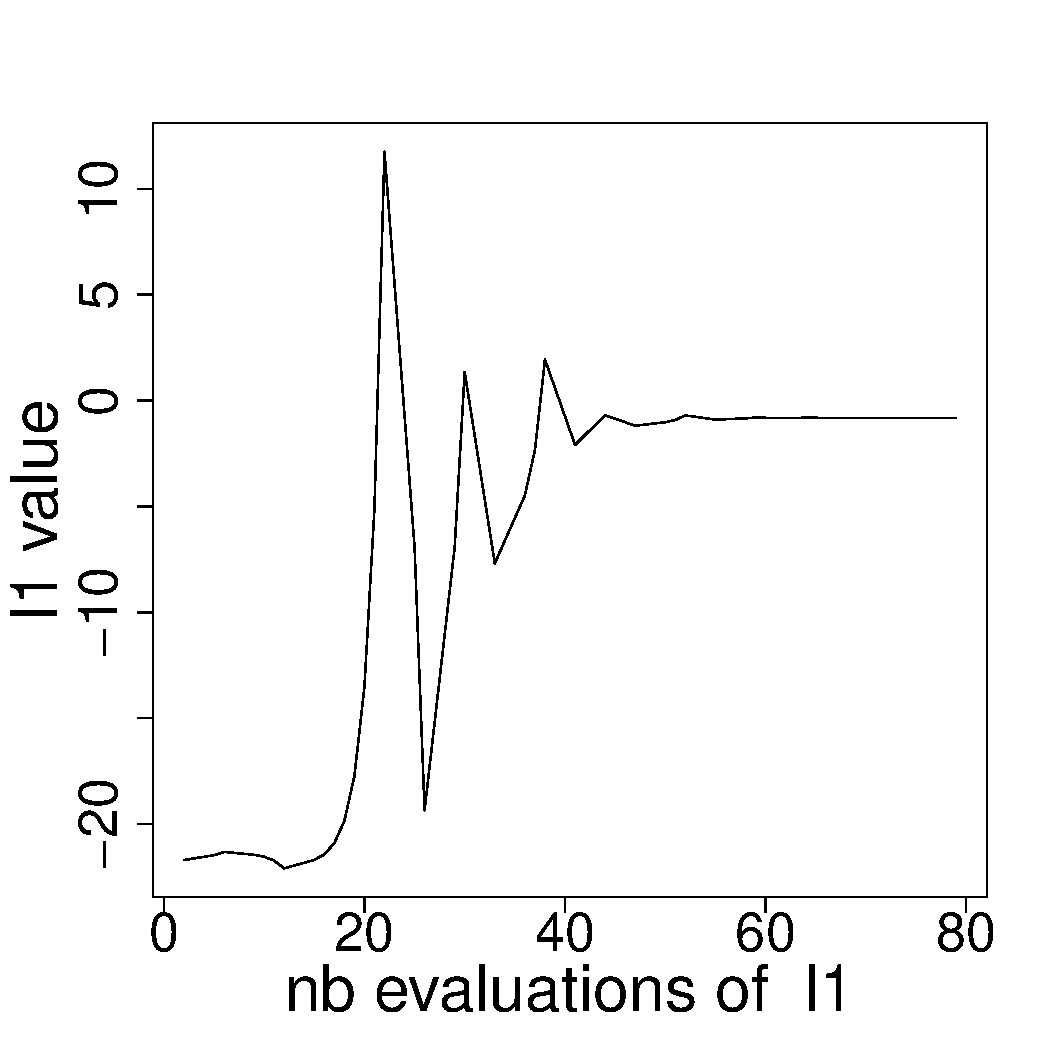
\includegraphics[width=\textwidth]{./R_figs/generated/l1_one_run}
		%\vspace{-20pt}
		\label{alexandrov_res_one:l1}
	\end{subfigure}
	\begin{subfigure}[b]{0.4\textwidth}
		\centering
		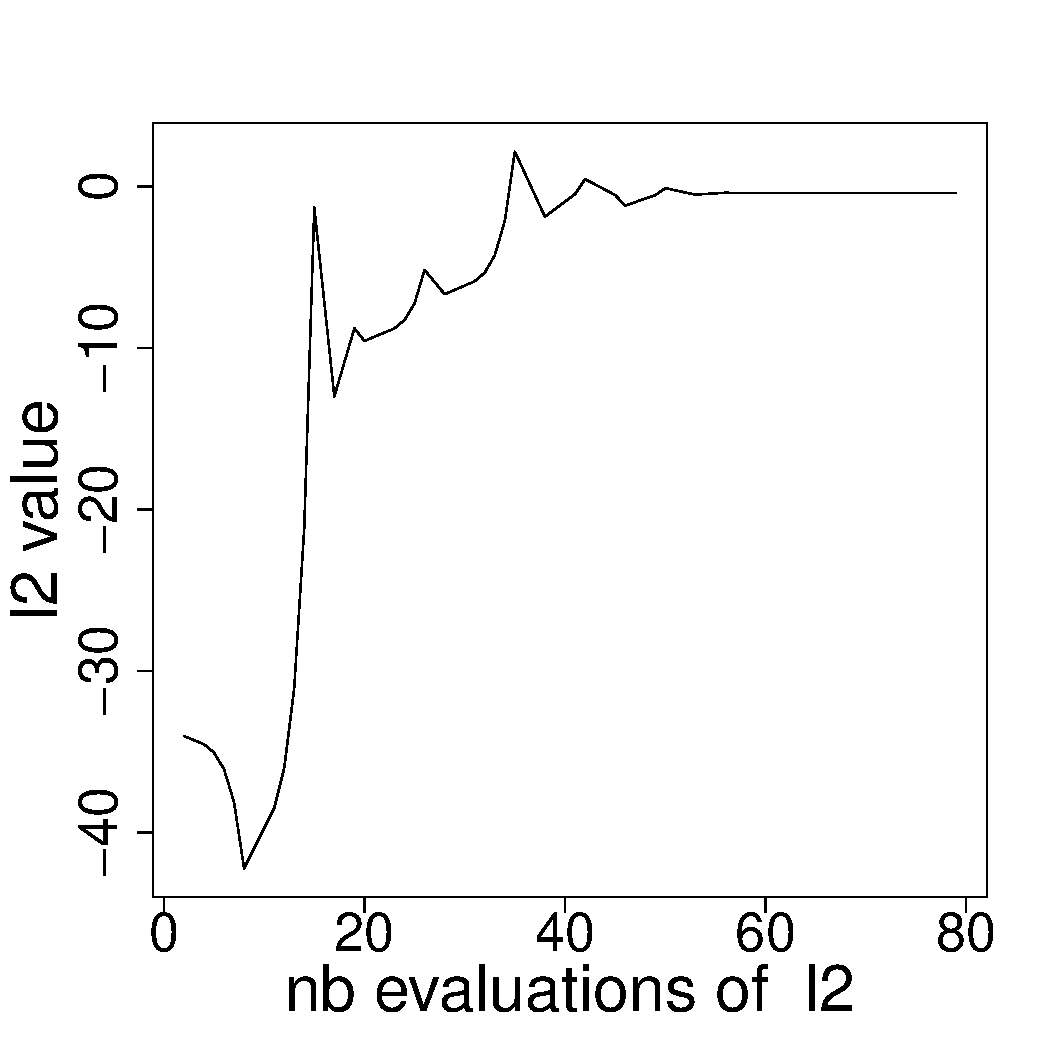
\includegraphics[width=\textwidth]{./R_figs/generated/l2_one_run}
		%\vspace{-20pt}
		\label{alexandrov_res_one:l2}
	\end{subfigure}
	\vspace{-20pt}
	\\
	\begin{subfigure}[b]{0.4\textwidth}
		\centering
		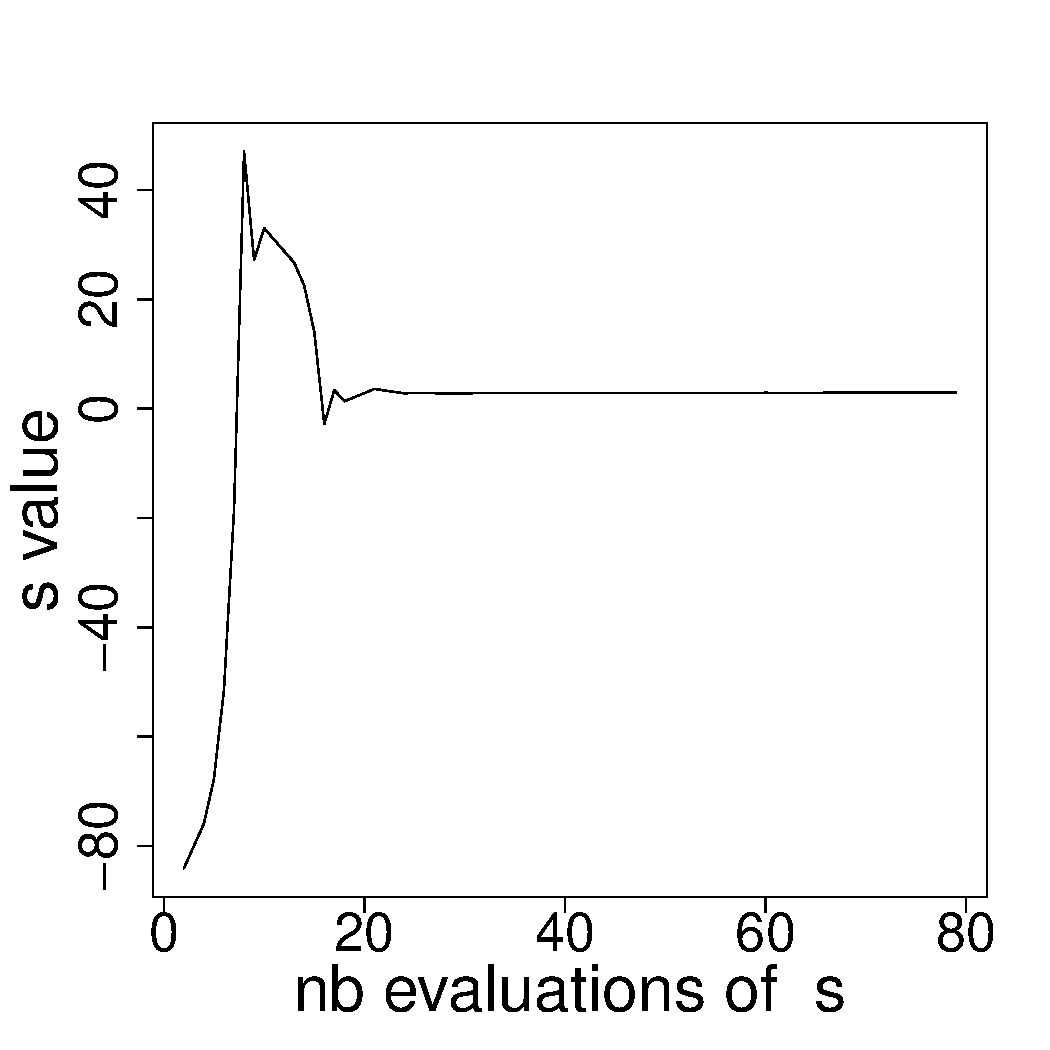
\includegraphics[width=\textwidth]{./R_figs/generated/s_one_run}
		%\vspace{-20pt}
		\label{alexandrov_res_one:s}
	\end{subfigure}
	\begin{subfigure}[b]{0.4\textwidth}
		\centering
		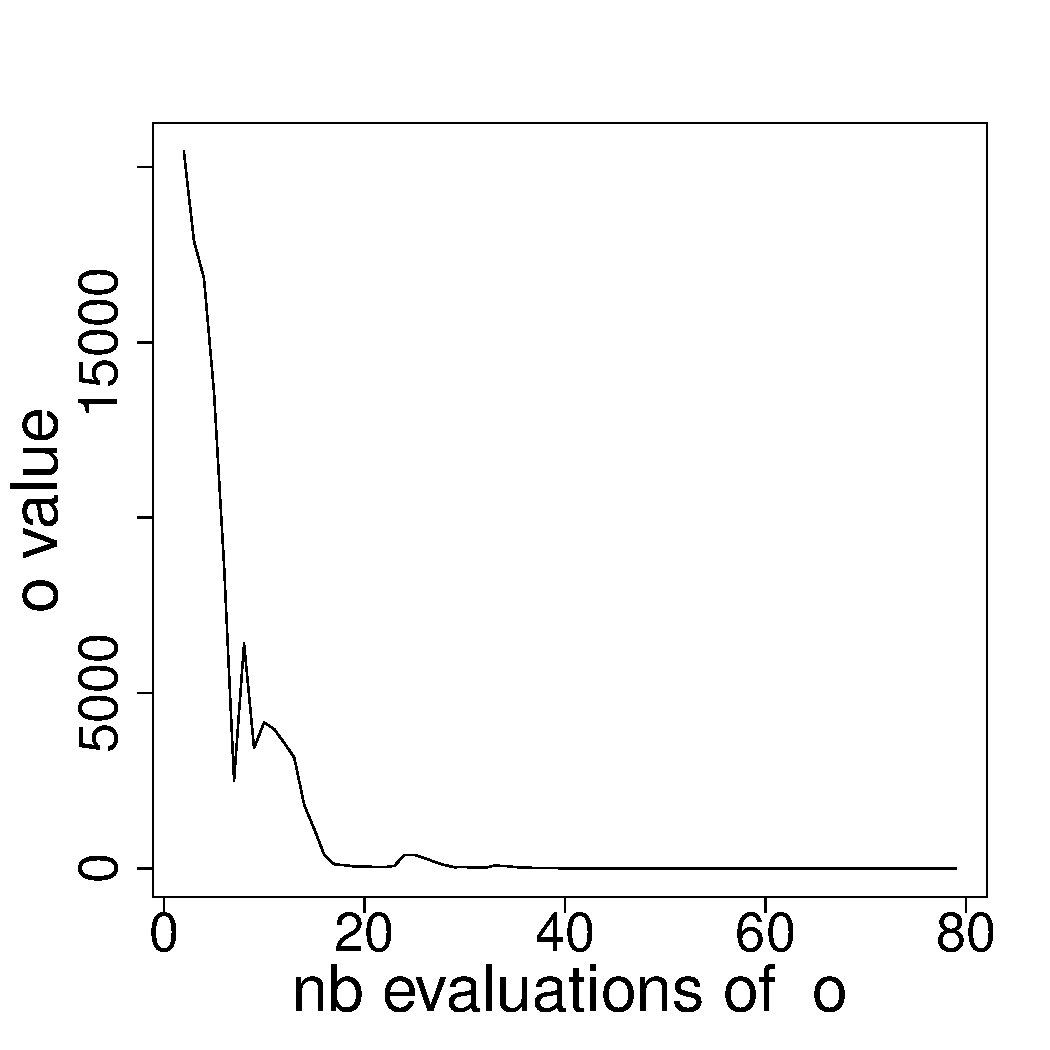
\includegraphics[width=\textwidth]{./R_figs/generated/o_one_run}
		%\vspace{-20pt}
		\label{alexandrov_res_one:o}
	\end{subfigure}
	
	\caption{Alexandrov agents behavior}
	\label{alexandrov_res_one}

\end{figure}

\begin{wrapfigure}{R}{0.4\textwidth}
	%\vspace{-50pt}
    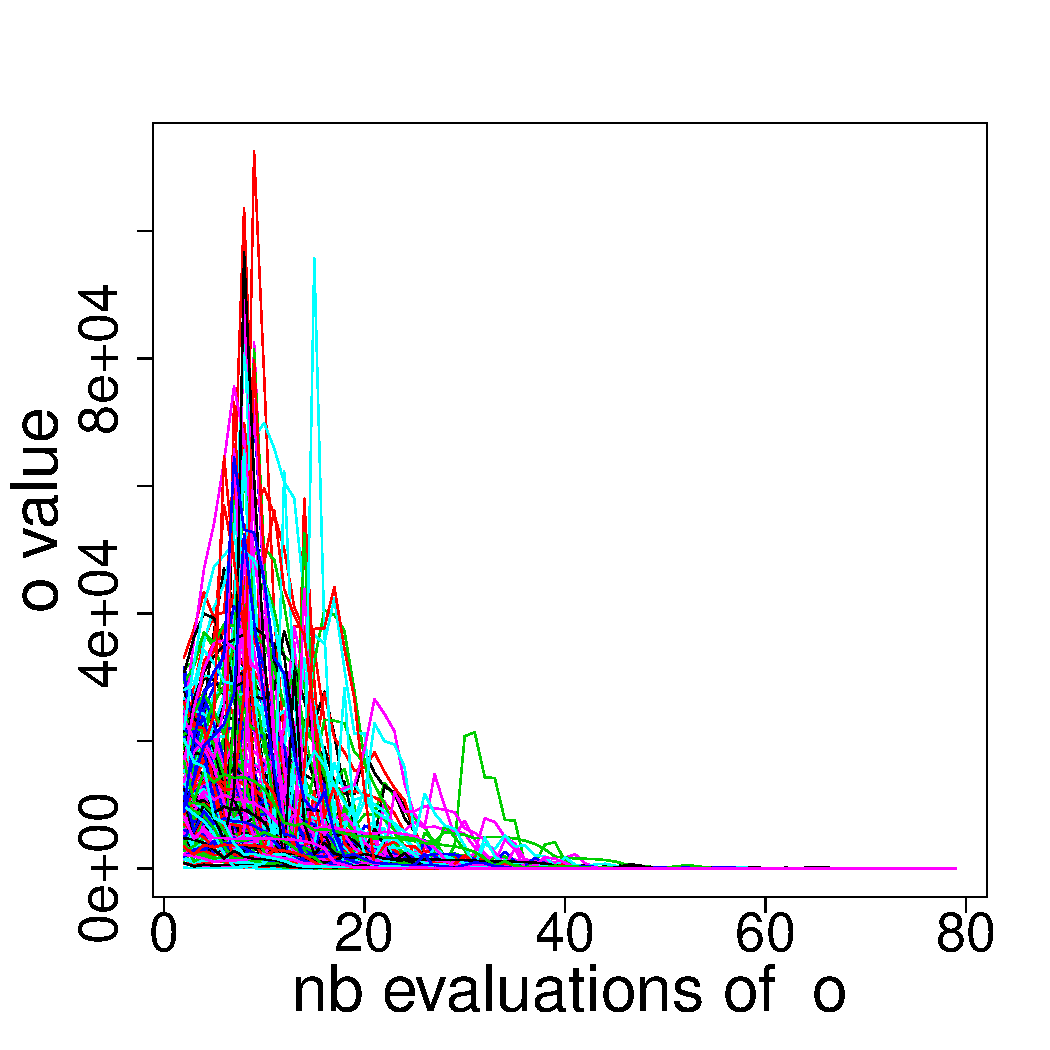
\includegraphics[width=0.4\textwidth]{./R_figs/generated/o}
	\caption{Convergence of the Alexandrov objective for 100 random starting points}
	\label{alexandrov_res}
	%\vspace{-25pt}
\end{wrapfigure}

Our first test case is inspired from an academic example taken in literature by Alexandrov and al\cite{alexandrov2002analytical}. This simple example presents some of the commons characteristics of MDO problems, such as interdependent disciplines and multiple criteria. In the original article, the example was used to illustrate some properties of Collaborative Optimization, which we presented earlier, in terms of reformulation. While the paper only gave the structure of the problem, we adapted it with meaningful values and equations.
The mathematical formulation of the problem and the corresponding agent graph can be seen in \figurename \ref{alexandrov}. Interestingly, the NDMO representation is quite similar to the one adopted by the original authors of the problem.

On \figurename \ref{alexandrov_res_one}, the behavior of the \emph{design variables} agents l1, l2 and s, as well the evolution of the objective, can be observed on one instance of the problem with random starting points. On \figurename \ref{alexandrov_res}, we show the evolution of the objective over 100 iterations with  starting points  for each \emph{design variable} randomly drawn over the interval [-100; 100]. We can see how the system converges towards the same optimum despite the wildly different initial conditions.

\section{Other Experiments}

We now briefly present results we obtained on two others test cases, the Turbofan problem and Viennet1. For each case, the system was executed 100 times with random starting points for each \emph{design variable}.

\subsection{Turbofan Problem}

The turbofan problem we introduced in \figurename \ref{turbofan} is a based on a real-world optimization problem, albeit simplified for demonstration purpose, concerning the conception of a turbofan engine.

As stated before, the problem concerns two \emph{design variables} $pi\_c$ and $bpr$. $pi\_c$ is defined inside the interval [20-40] and $bpr$ inside [2-10]. The model produces three variables $Tdm0$, $s$ and $fr$.
The problem has two objectives, maximizing  $Tdm0$ and minimizing $s$, under the constraint \(s \leq 155\) and \(fr \geq 4\).
The main interest and difficulty of this problem is the existence of two contradictory objectives.
As we can see on \figurename \ref{snecma_res}, the system consistently converges toward the same optimal solution.

\begin{figure}[h]
	\begin{subfigure}[b]{0.49\textwidth}
		\centering
		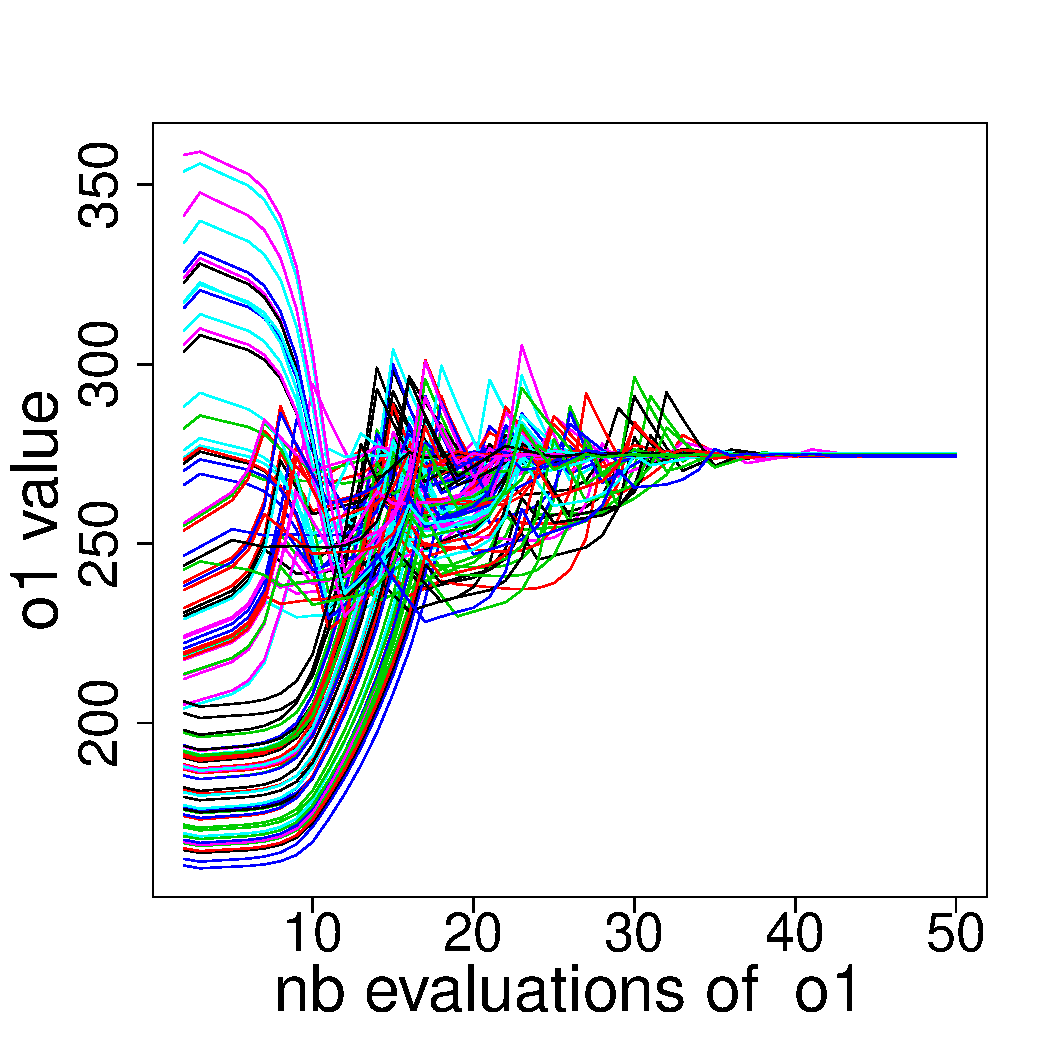
\includegraphics[width = \textwidth]{./R_figs/generated/o1}	
	\end{subfigure}
	\hfill%for spacing
	\begin{subfigure}[b]{0.49\textwidth}
		\centering
		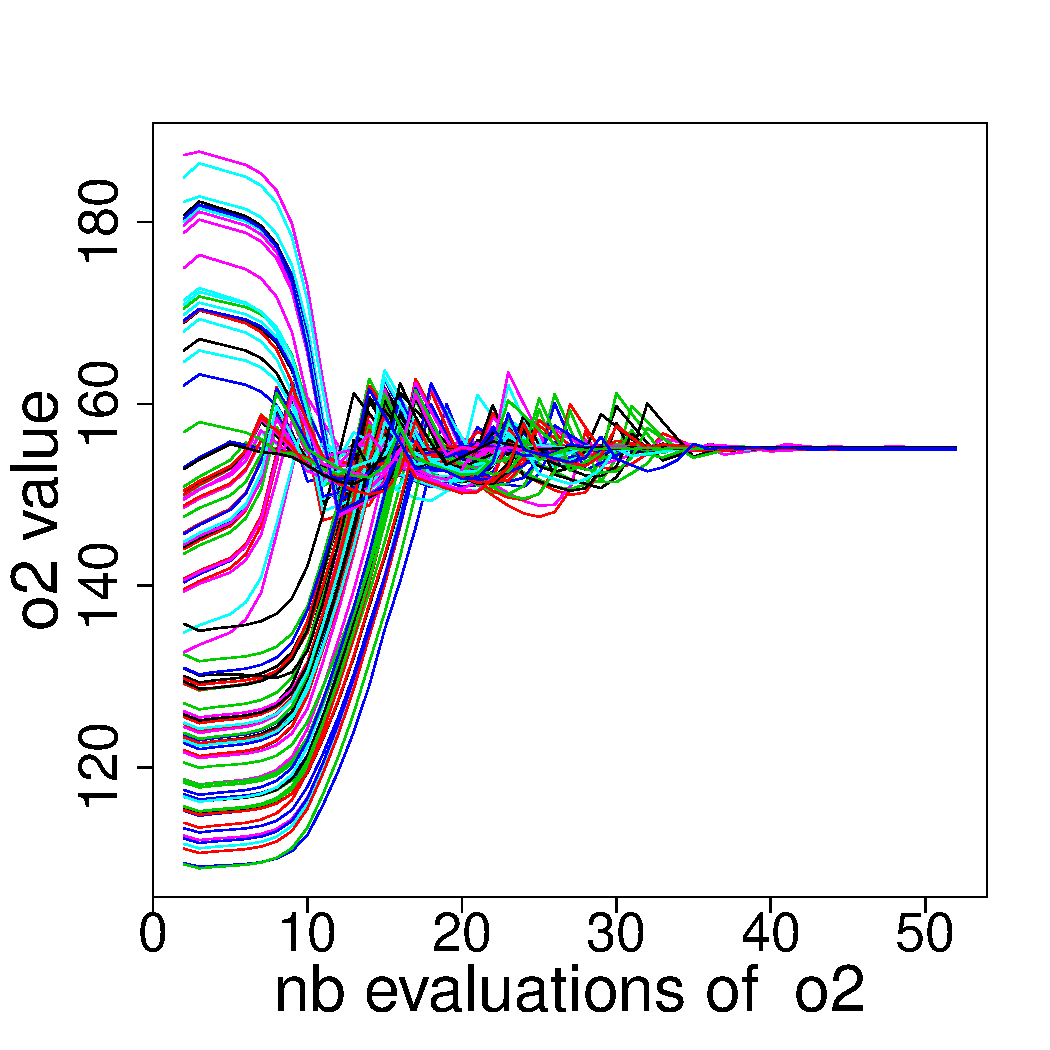
\includegraphics[width = \textwidth]{./R_figs/generated/o2}	
	\end{subfigure}
	\caption{Convergence of the Turbofan objectives for 100 random starting points}
	\label{snecma_res}
\end{figure}

\subsection{Viennet1}

The Viennet1 test case is part of a series of problems proposed in \cite{viennet1996multicriteria} to evaluate multi-criteria optimization techniques. This problem involves three objectives. Its analytical formulation is:


$$\text{Minimize } o1 = x^2 + (y-1)^2 \text{, } o2 = x^2 + (y+1)^2 \text{ and } o3 = (x-1)^2 + y^2 +2\\$$
$$\text{where } x, y \in  [-4;4]
$$

\figurename \ref{viennet_res} illustrates the convergence of the system towards a valid solution.


\begin{figure}[h]

	\begin{subfigure}[b]{0.32\textwidth}
		\centering
		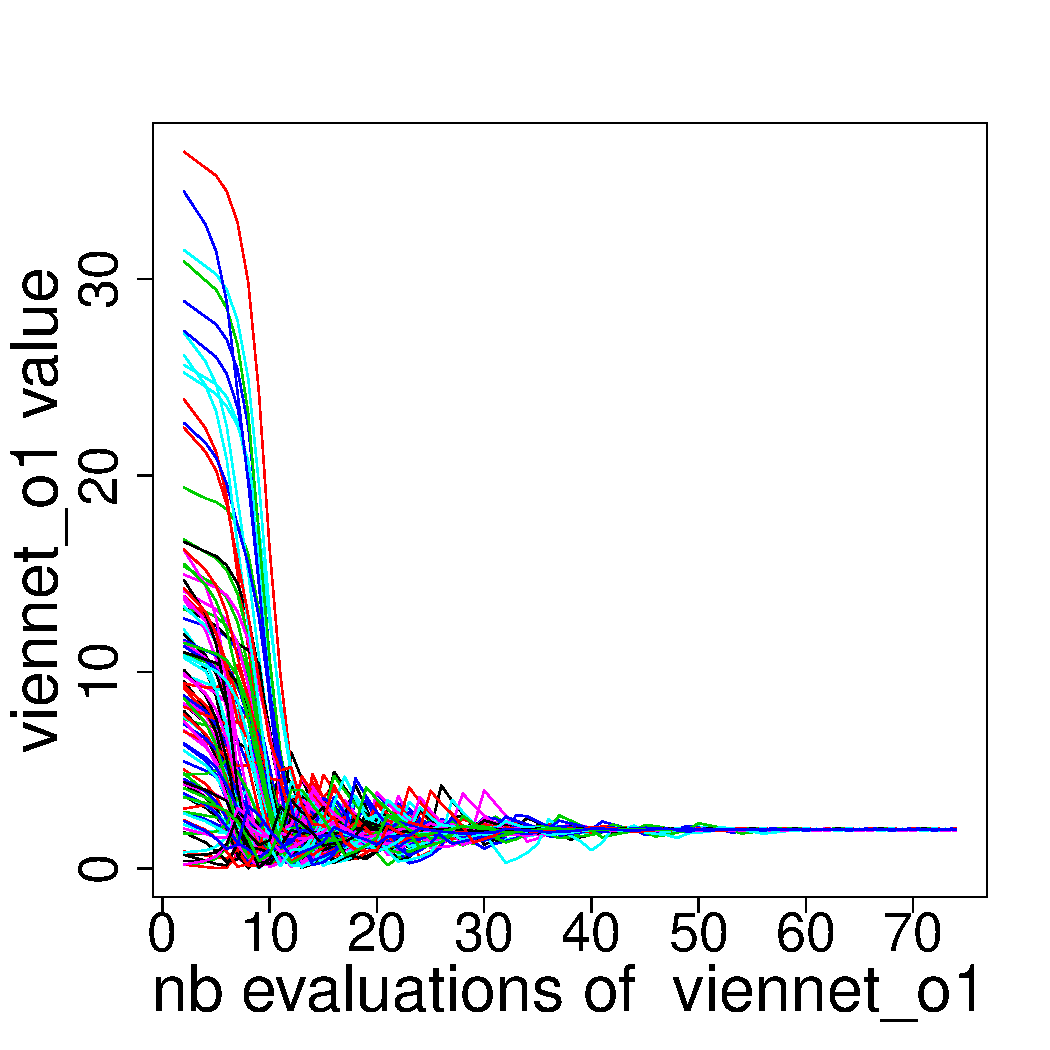
\includegraphics[width = \textwidth]{./R_figs/generated/viennet_o1}	
	\end{subfigure}
	\hfill%for spacing
	\begin{subfigure}[b]{0.32\textwidth}
		\centering
		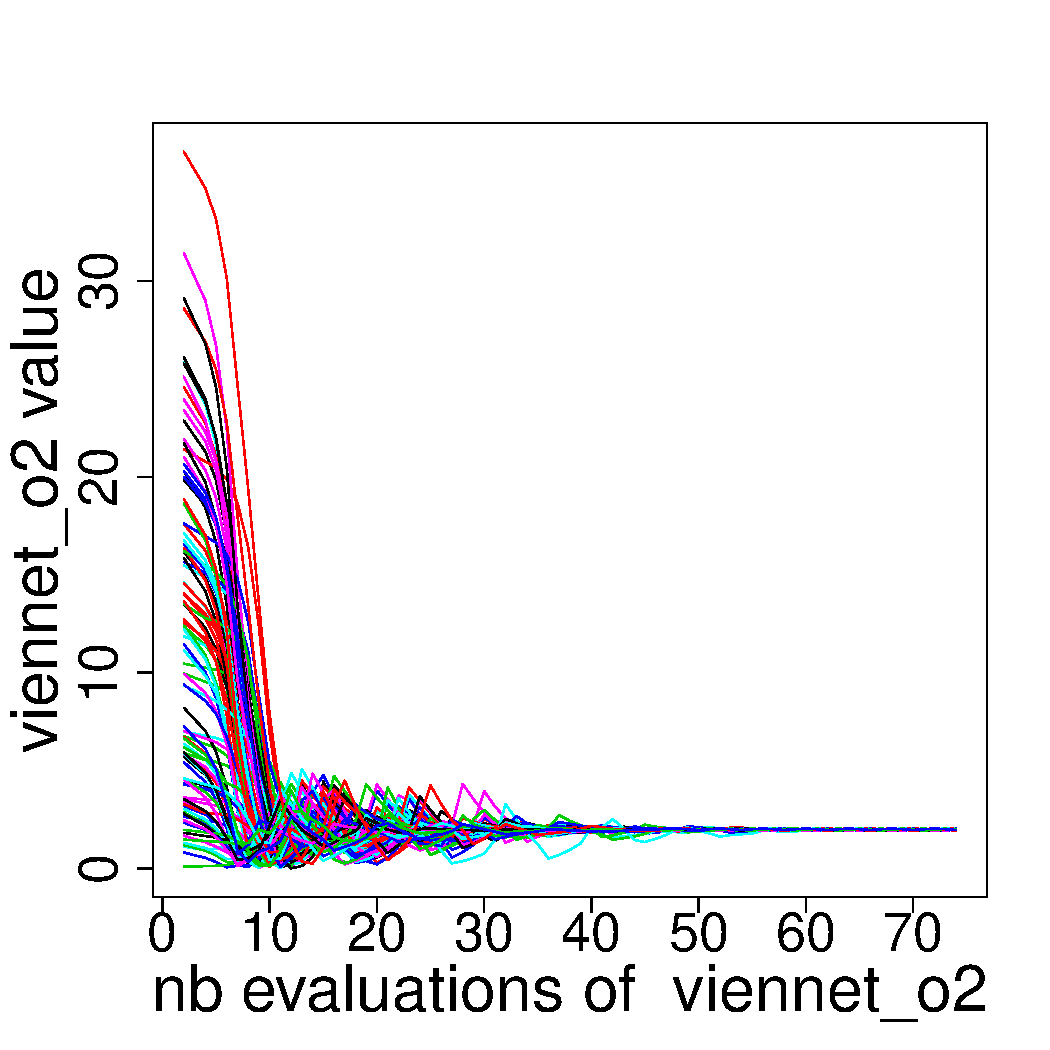
\includegraphics[width = \textwidth]{./R_figs/generated/viennet_o2}	
	\end{subfigure}
	\hfill%for spacing
	\begin{subfigure}[b]{0.32\textwidth}
		\centering
		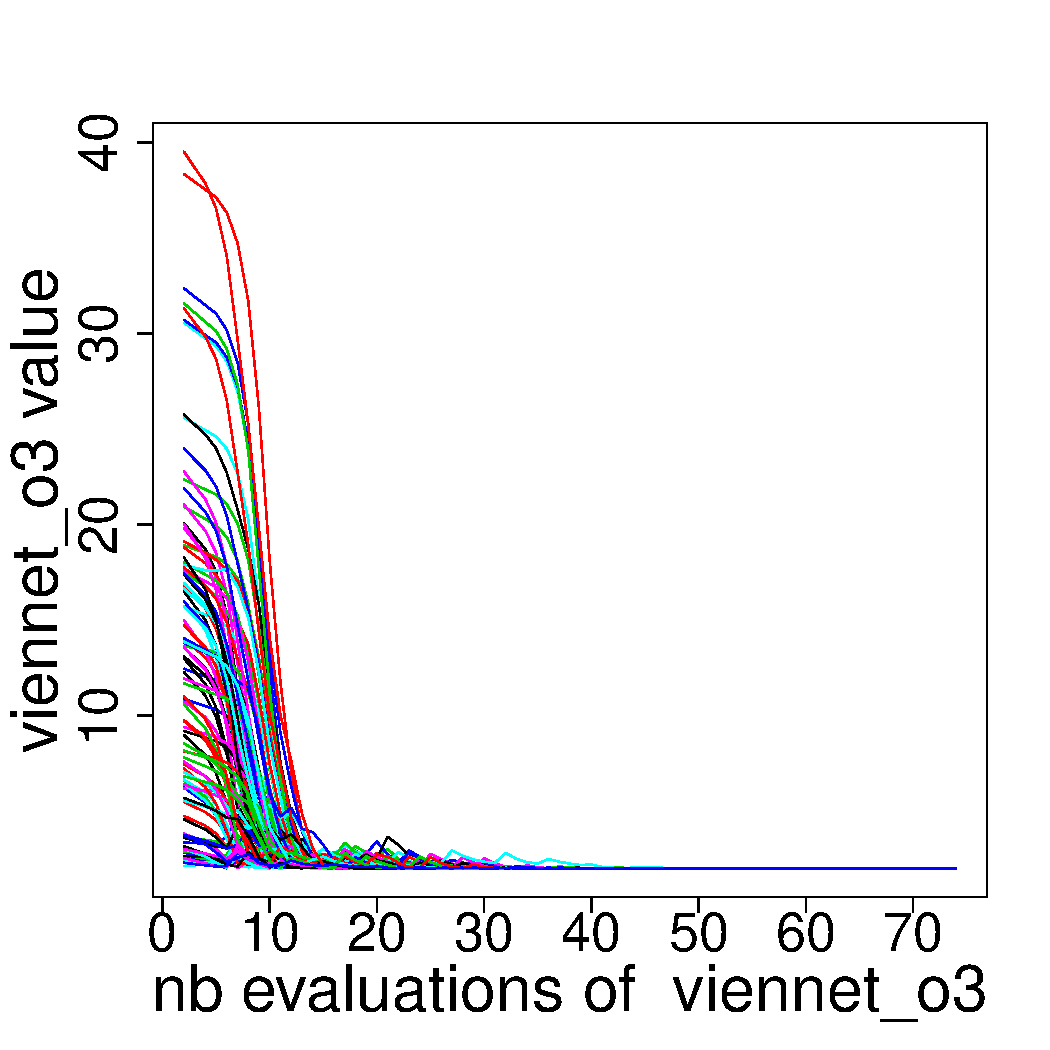
\includegraphics[width = \textwidth]{./R_figs/generated/viennet_o3}	
	\end{subfigure}
	\caption{Convergence of Viennet1 objectives for 100 random starting points}
	\label{viennet_res}
\end{figure}

\subsection{Rosenbrock's valley}

Rosenbrock's valley is non-convex function commonly used to test convergence performances. The results presented here are for the two-dimensional version of the problem with a definition domain of [-5; 5] for each \emph{design variable}.
The analytical formulation of this problem (for two dimensions) is 
$$\text{Minimize } f(x,y) = (1-x)^2 + 100(y - x^2)^2$$

\begin{wrapfigure}{R}{0.5\textwidth}
    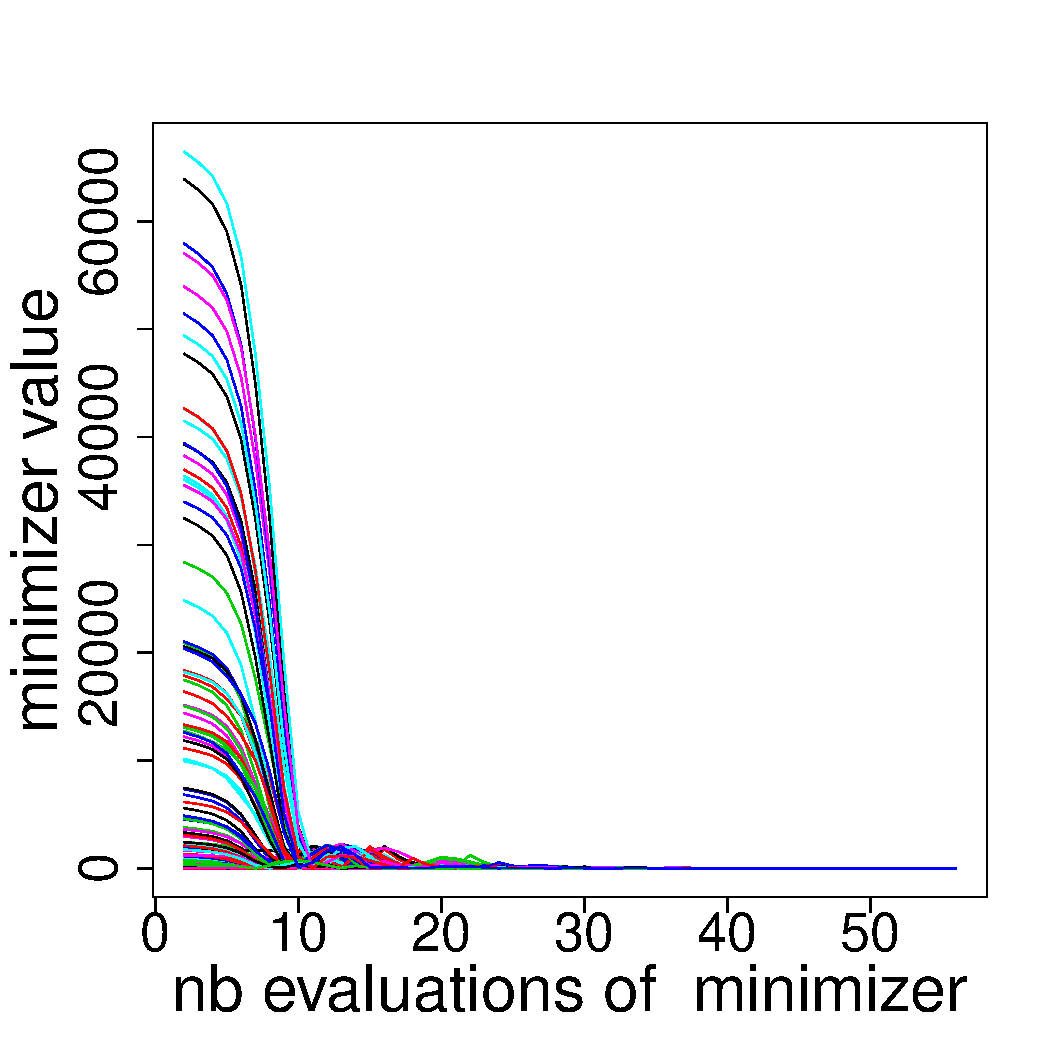
\includegraphics[width = 0.5\textwidth]{./R_figs/generated/minimizer}	
	\caption{Convergence of Rosenbrock objective for 100 random starting points}
	\vspace{-20pt}
\end{wrapfigure}

\chapter{Large Tests Cases and Comparisons with Existing Methods}

\section{Preliminary Aircraft Design}

\section{Snecma 2}

\section{Benchmarks}

\chapter{Generated Test Cases and Scalability}

In this section we present some measures we established in regard of the scalability performances of our MAS. [[TOCHANGE if spring networks are integrated]] For this part of the experiments we were not concerned with the optimization performances of the system, but more with its capability to handle large agent graphs without suffering from performances degradation.

In order to realize our experiments, we required a large number of test cases of several sizes and comparable complexity.  Since such repository of continuous optimization problems is not readily available, we worked on a way to automatically generate them. To this end, we took advantage of the fact that, as demonstrated with our NDMO modeling, an optimization problem can be represented as a graph. Consequently it is possible to use well-known graph generation techniques and directly generate problem graphs.

We propose a very simple method to generate simple problem graphs. First we use a graph generation algorithm to generate a directed graph of size $n$. The nodes of this graph represent the variables of the problem and the arcs their dependencies. If a node is not the head of any arc (\emph{i.e.} there is no arc going to this node), it is a design variable, otherwise it is an output variable.\\
The next step is to insert models. As we stated, the optimization problem in itself is of little importance in this part. Consequently our only requirement for the model is that they must be able to take an arbitrary number of inputs and produce one output. In our experiments we used a simple \emph{Sum} function. For each output variable, we insert a node representing the model in the graph. The links going to the output variable node are redirected to the model node, and a link going from the model node to the output node is create.\\
After this step, criteria are randomly added to variable nodes. In our experiments, we given a 20\% probability of a variable node  to be linked to a criterion, with half the chance for the criterion to be an objective and half the change for it to be a constraint. Once more, in order to simplify the problem generation, all objectives are about minimizing the variable, and are constraints are about having the variable higher of equal to zero.

The generation method is summarized in \ref{algo_graph_generation}. After all these steps, the graph is a valid [[(if not useful)]] NDMO graph and can be directly transformed into an agent graph.

\begin{algorithm}
\caption{Problem graph generation}
\label{algo_graph_generation}
	$n \leftarrow$ initialization number
	$G(nodes, arcs) \leftarrow GraphGenerator(n)$\;
			
		\ForEach{$currentNode \in G.nodes$}{
			tag($currentNode$, \enquote{variable})\;
			$enteringArcs \leftarrow \{arc \in G.arcs, isHeadOf(arc, currentNode)\}$
			\If{$enteringArcs \neq \emptyset$}{
				\tcp{$currentNode$ is an output variable}
				$modelNode \leftarrow $ new node\;
				tag($modelNode$, \enquote{model})\;
				$G$.add($modelNode$)\;
				$G$.createArcBetween($modelNode$, $currentNode$)\;
				\ForEach{$arc \leftarrow enteringArcs$}{
					$tailNode \leftarrow arc.tail$\;
					$G$.removeArc($arc$)\;
					$G$.createArcBetween($tailNode$, $modelNode$)\;
				}
			}
			\;
			\tcp{check for criteria}			
			$rand \leftarrow drawRandomNumber()$\;		
			\If{$rand \leq	 criteriaProba$}{		
				$critNode \leftarrow$ new node\;
				$G$.createArcBetween($currentNode$, $critNode$)\;
				\eIf{$rand \leq drawRandomNumber/2$}{
					tag($critNode$, \enquote{objective})\;				
				}{
					tag($critNode$, \enquote{constraint})\;
				}
			}		
		}

\end{algorithm}

It must be noted that the final size of problems generated by this algorithm is not fixed, and can be significantly larger than the initialization value $n$. However problems produced using the same initialization number and the same graph generator are of comparable sizes.

We used graph generators proposed by the GraphStream library \footnote{\url{http://www.graphstream-project.org/}}. On \figurename{} \ref{graph_generation_examples} some examples of graphs produced using these generators are visualized using GraphStream visualization tools. It should be noted that, because  of the modifications we apply on the graph after it is created using the generator, the final agent graph does not necessarily respect the properties of the initial graph , however we can see on \figurename{} \ref{graph_generation_examples} that, the modifications we apply do not radically modify the characteristic topologies of the different graph types.
 
\begin{figure}
\centering
	\begin{subfigure}[b]{0.45\textwidth}
		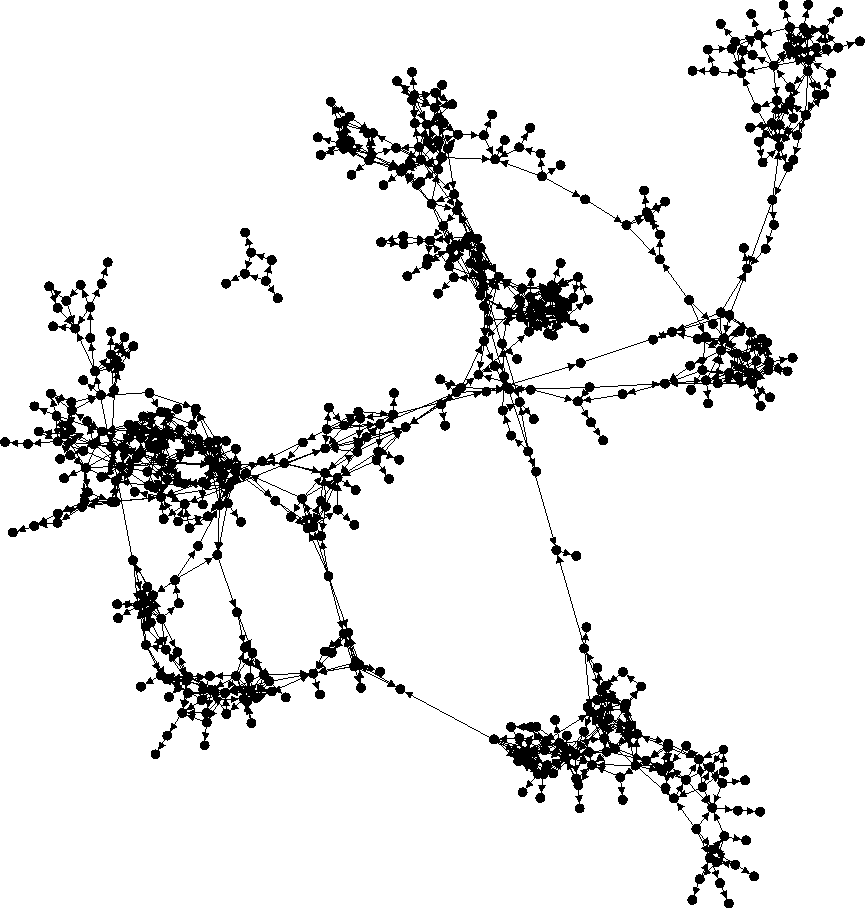
\includegraphics[width=\textwidth]{graph_random_euclid_1}
		\caption{Random Euclidean graph example 1.}\label{generatedgraphs:rand1}
	\end{subfigure}
	\begin{subfigure}[b]{0.45\textwidth}
			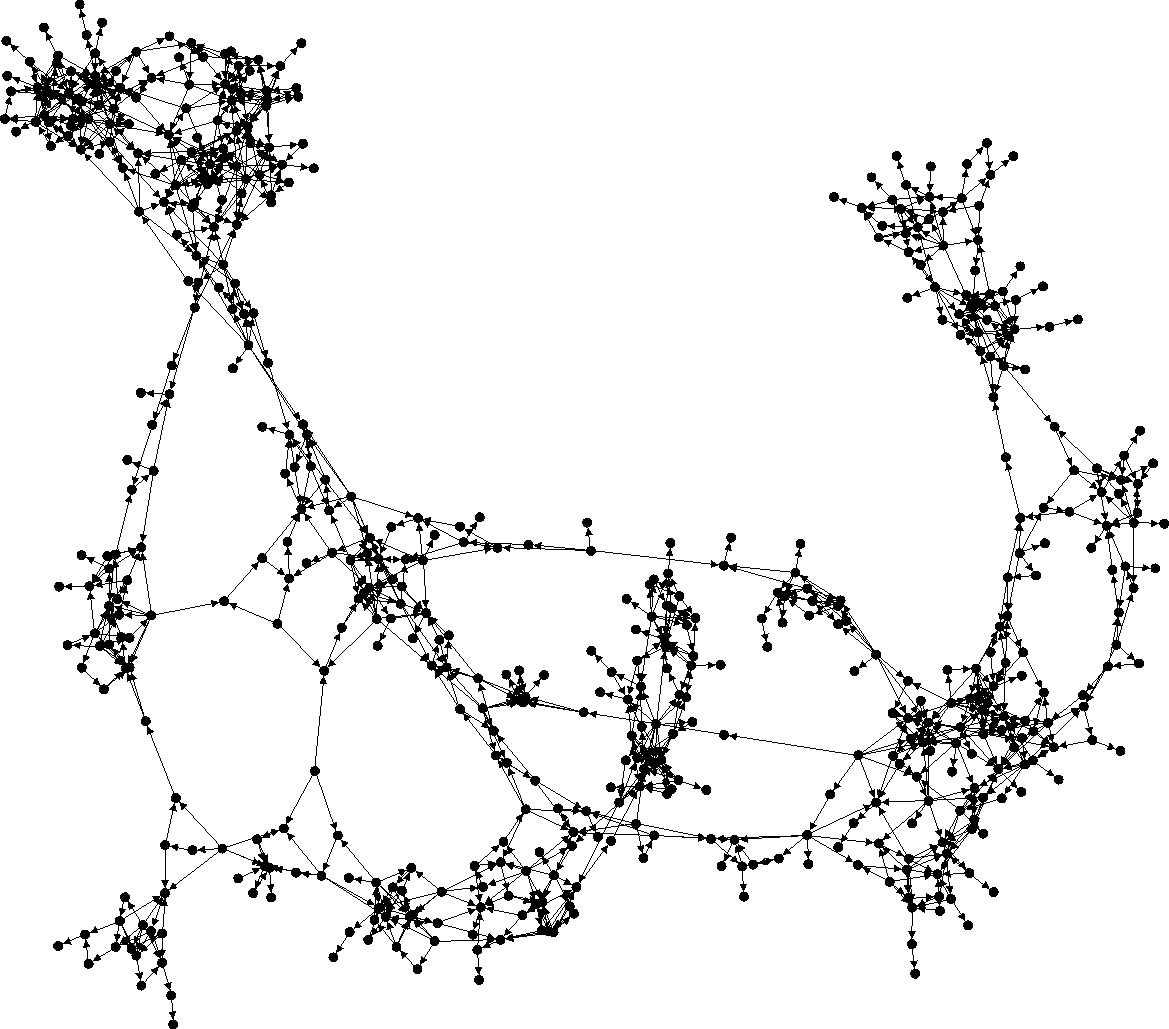
\includegraphics[width=\textwidth]{graph_random_euclid_2}
		\caption{Random Euclidean graph example 2.}\label{generatedgraphs:rand2}
	\end{subfigure}
	
	\begin{subfigure}[b]{0.45\textwidth}
		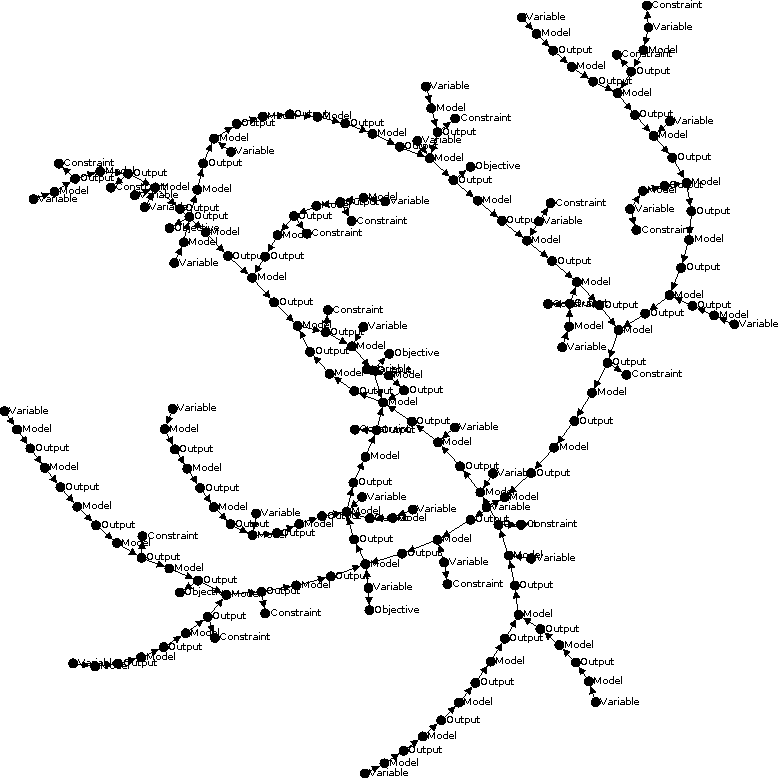
\includegraphics[width=\textwidth]{graph_SW_1}
		\caption{Small-World graph example 1.}\label{generatedgraphs:sw1}
	\end{subfigure}
	\begin{subfigure}[b]{0.45\textwidth}
			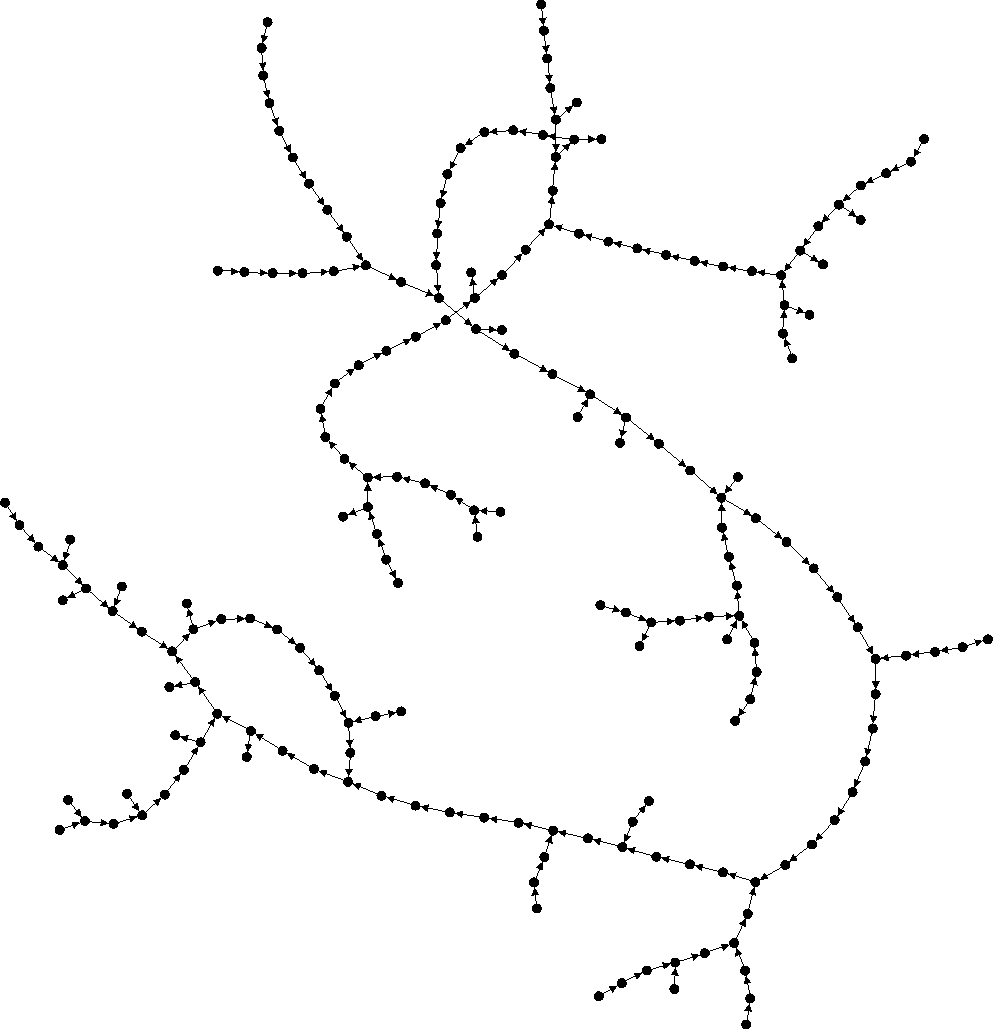
\includegraphics[width=\textwidth]{graph_SW_2}
		\caption{Small-World graph example 2.}\label{generatedgraphs:sw2}
	\end{subfigure}

\caption{Examples of graph generation.}
\label{graph_generation_examples}
\end{figure}

Before discussing the results we obtained, let us add a word of warning concerning measuring real-time performances of java applications (java being the programming language used to implement our prototype). The Java Virtual Machine (JVM), which executes java programs, applies a lot of complex optimization steps \emph{during} the execution process. Consequently making some precise and non-biased measurements can be hazardous.\\
Regarding our experiments, we tried to mitigate possible bias by taking the two following precautions:
\begin{compactitem}
\item before running the measured experiments, running multiple problems whose results were discarded, in order to \enquote{heat} the JVM and allowing it to apply its optimization procedures beforehand.
\item running the different experiments multiple times and in different orders, to \enquote{spread} the benefits of possible optimizations happening at runtime.
\end{compactitem}
We believe that these precautions are sufficient to obtain sufficiently meaningful results. Nevertheless, the reader should be warned not to consider the presented values as exact measurements of the system performances.

On \figurename{} \ref{generated_perfo:time} are presented the results of the execution time of problems of different sizes. We generated agent graphs of different sizes using both Small-Word and Random Euclidean algorithms. For each size and each generator we create 20 instances of problems. On the figure are presented the mean time needed for all the agents of the problem to execute one behavior cycle. Interestingly, while the time performances in regard of small-world based problems graphs increase linearly with the size of the problems, the time needed in the case of random problem graphs seems to increase exponentially.\\
This seemingly poor performance can however easily be explained by looking at \figurename{} \ref{generated_perfo:degree}, on which are shown the mean degree (that is, the number of arcs entering of exiting a node) of the nodes in each generated problems. We can see, that, whatever the size of the problem, the mean degree of a node in Small-World problems is mostly constant. However, in the case of Random Euclidean graphs, the mean degree increases linearly with the size of the problem. Consequently, the exponential increase in time regarding Random Euclidean graphs can be explained by the conjugated effects of the increase in number of agents and the increase of the neighborhood size of the agents (whose impact in the behavior algorithm complexity has been exposed in section \ref{NCS_pres}).

\begin{figure}
\centering

	\begin{subfigure}[b]{0.45\textwidth}
		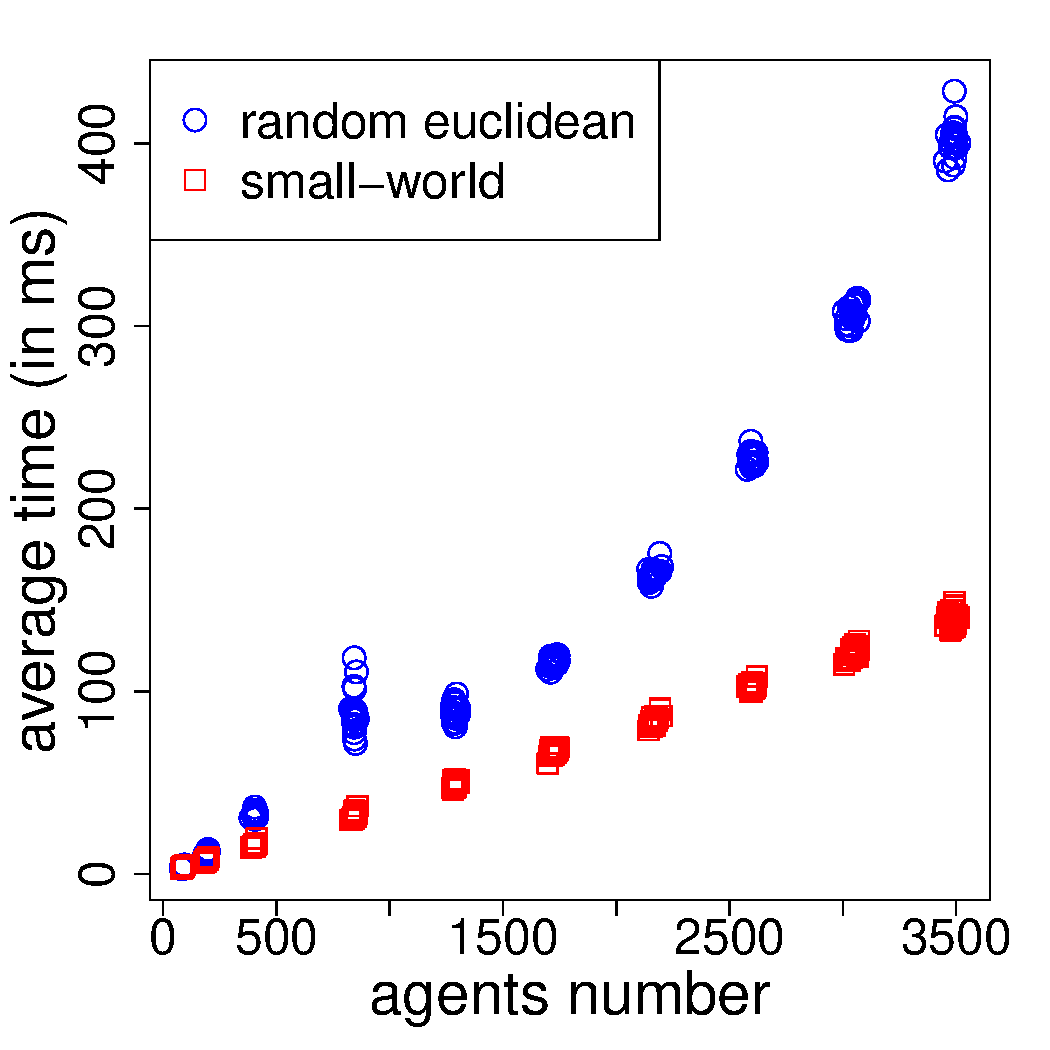
\includegraphics[width=\textwidth]{R_figs/graph_problems/comp_time_by_size}
		\caption{Average time for a step.}\label{generated_perfo:time}
	\end{subfigure}
	\begin{subfigure}[b]{0.45\textwidth}
			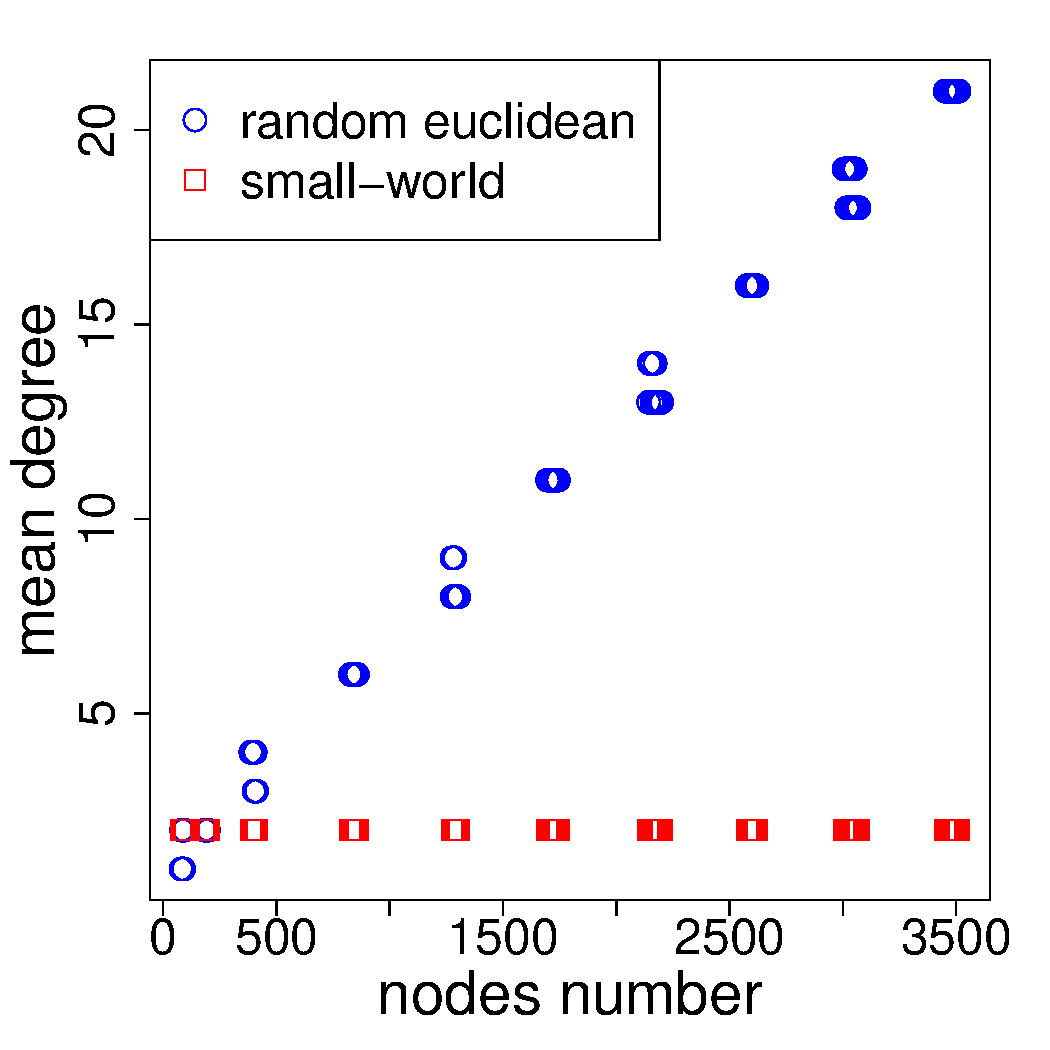
\includegraphics[width=\textwidth]{R_figs/graph_problems/comp_degree_by_size}
		\caption{Mean degree of nodes.}\label{generated_perfo:degree}
	\end{subfigure}

\caption{Time performances by MAS size.}
\label{generated_perfo}
\end{figure}

In order to corroborate this analysis, we studied the impact increasing the nodes degree has on the execution time of the MAS. On \figurename{} \ref{experiment_degrees}, we show the results of another experiment using agent graphs generated using a Barabasi-Albert generator, which has the advantage of being able to easily generate graphs with different mean degree sizes at the cost of only a slight increase of node numbers. On the figure is shown the average time for all the agents to make a behavior cycle in function of the mean degree of the agents (using Barabasi-Albert based graphs of sizes between 510 and 550 nodes). We can see that the neighborhood size of the agents (the degree of the node) has the predicted effect on the time needed by the agents to execute their behavior.

\begin{figure}
\centering
	\begin{subfigure}[b]{0.45\textwidth}
		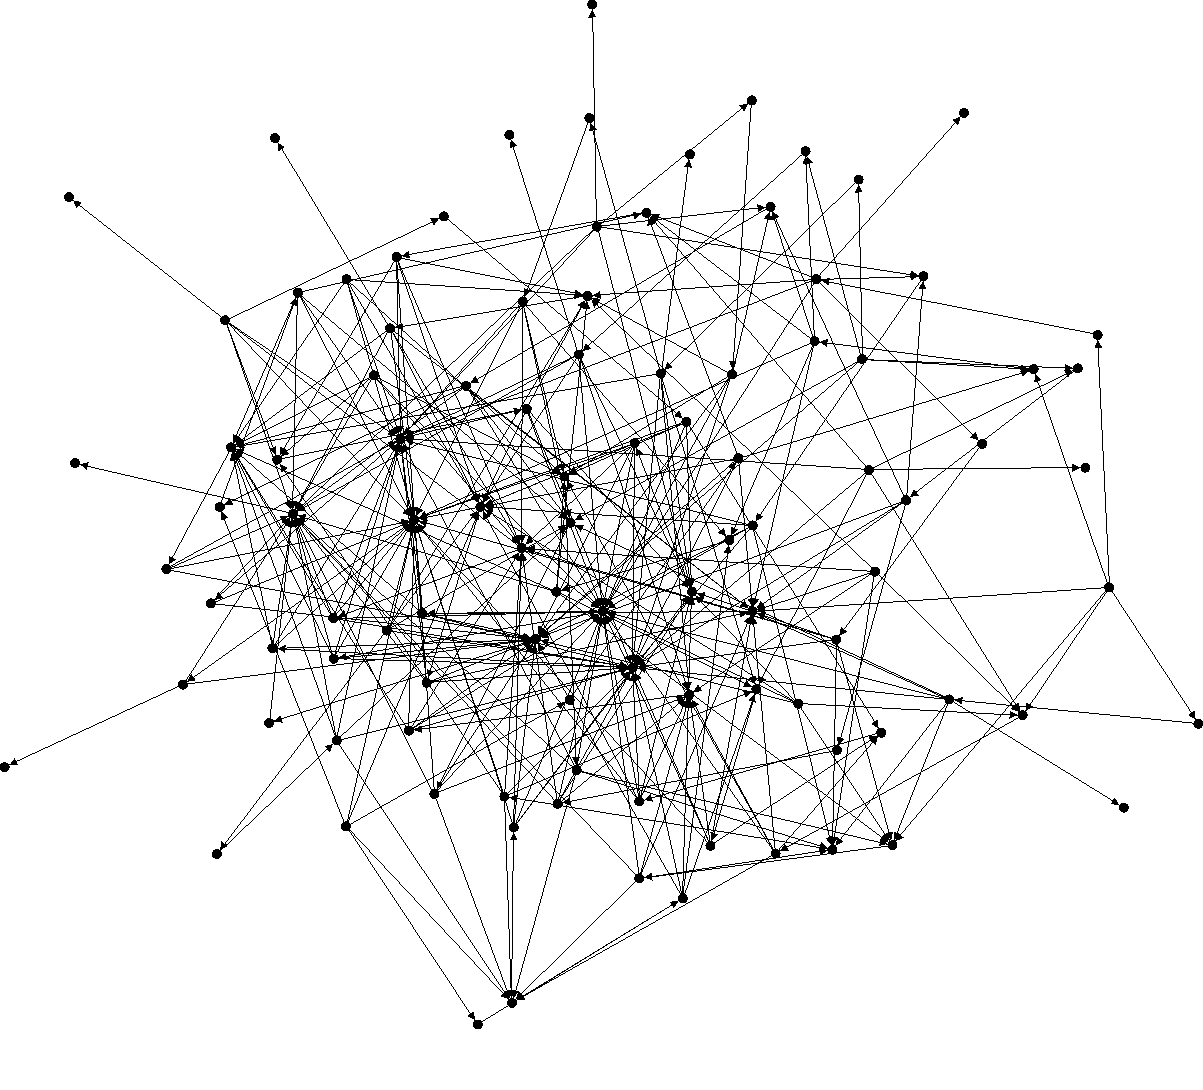
\includegraphics[width=\textwidth]{graph_barabasi_albert}
		\caption{Barabasi-Albert graph example.}\label{experiment_degrees:graph}
	\end{subfigure}
	\begin{subfigure}[b]{0.45\textwidth}
			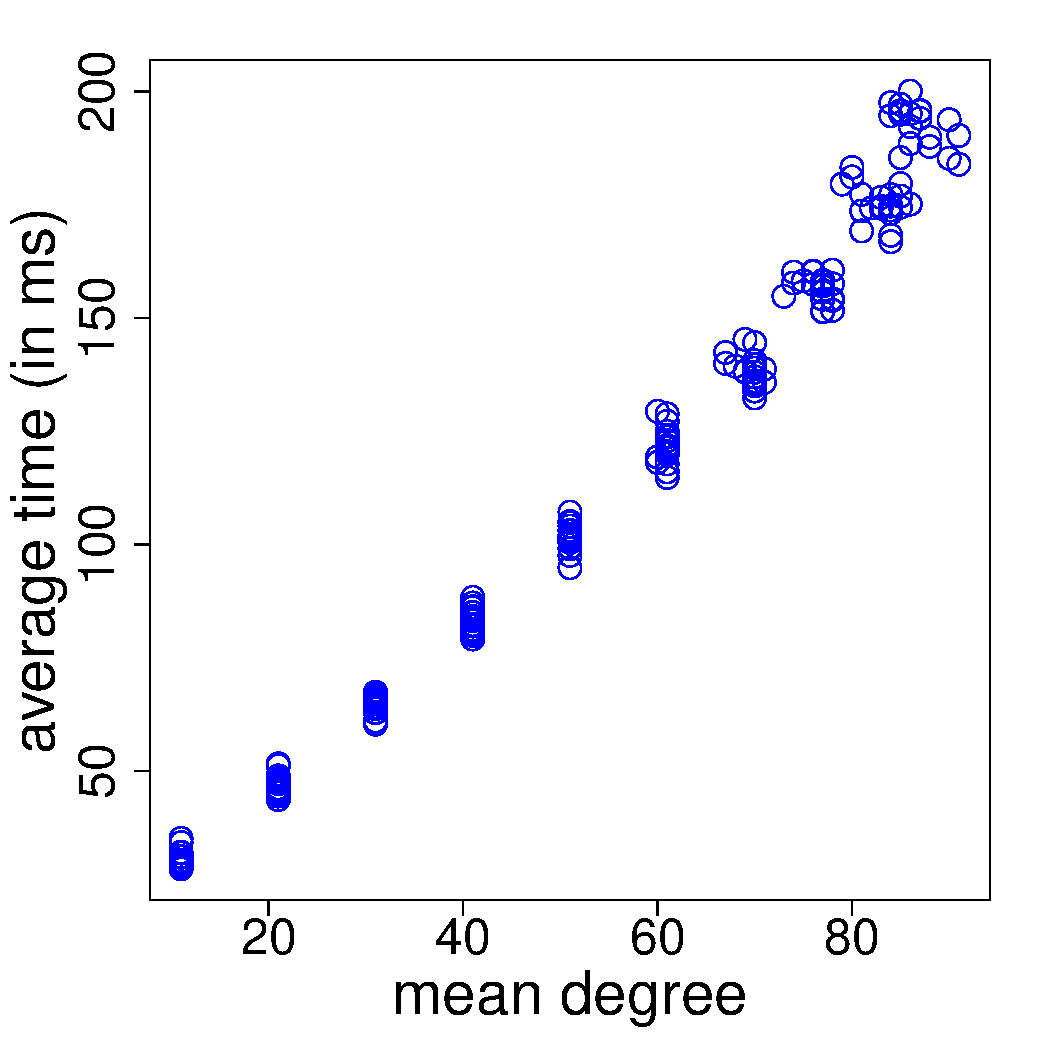
\includegraphics[width=\textwidth]{R_figs/graph_problems/comp_time_by_degree}
		\caption{Average time for a step (by mean degree).}\label{experiment_degrees:res}
	\end{subfigure}
\caption{Time performances by node degree.}
\label{experiment_degrees}
\end{figure}

Overall, we can conclude by observing these results that the time required for the agents to make a behavior cycle is not meaningfully impacted by the size of the problem. This property is an expected benefit of restricting the agents to local perception and decision process.

As an additional observation, some artifacts can be identified on \figurename{} \ref{generated_perfo:time} and  \figurename{} \ref{generated_perfo:degree}. \figurename{} \ref{generated_perfo:time} presents a strange \enquote{hump} for Random Euclidean graphs when the number of agents is around 800, while on \figurename{} \ref{generated_perfo:degree}, the mean degree of Random Euclidean graphs seems to follows a cyclic pattern, where the mean degree seem to be localized alternatively between one and two points. it should be noted that, while the first anomaly is observed when running our system, the second one is completely independent the behavior of the MAS an is simply a statistical analysis on the generated graph.\\
The first artifact could be explained by some of the possible evaluation pitfalls of measuring performances in java we presented at the start of the chapter, however we ran the experiments in several orders and observed the same phenomenon in each case.\\
Another possibility, which would explain both artifacts, would be a bias introduced in our algorithm to transform the generated graph into a valid NDMO agent graph. But we found no obvious link between our algorithm and the periodic nature of the second artifact.\\
A third explanation could be a potential bias in either the implementation of the Random Euclidean generator algorithm we use, or in the algorithm in itself.\\
In any case, we believe these two oddities not significant nor relevant enough to put in question the results we observed or the conclusions which can be drawn from them.


\chapter{Others Experiments}

\section{Optimization under Uncertainties}

\section{Adaptation to Perturbations}

\subsection{Perturbated Alexandrov}
 
On \figurename \ref{alexandrov_res_pert}, we can observe the reaction of the multi-agent system to a perturbation. During the solving of the previous experimentation on the problem, we changed the threshold of the constraint $s + l_1 \leq 1$ to $s + l_1 \leq -4$ (the change is indicated by a dotted line on the charts). The system dynamically adapts to the constraint changed and converges towards a new solution which satisfies the updated constraint.

\begin{figure}[]
\centering
  	\begin{subfigure}[b]{0.4\textwidth}
		\centering
		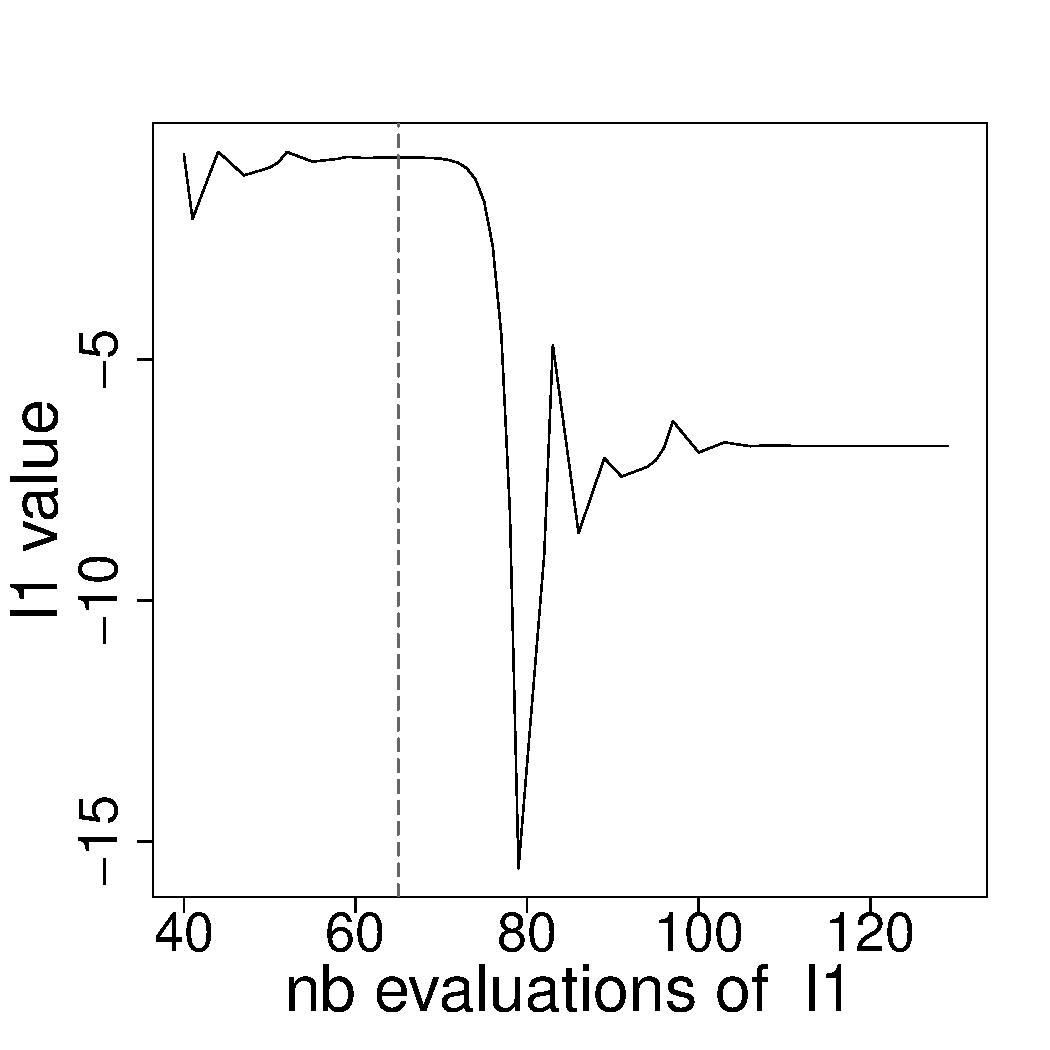
\includegraphics[width=\textwidth]{./R_figs/generated/l1_pertubated}
		%\vspace{-20pt}
		\label{alexandrov_res_pert:l1}
	\end{subfigure}
	\begin{subfigure}[b]{0.4\textwidth}
		\centering
		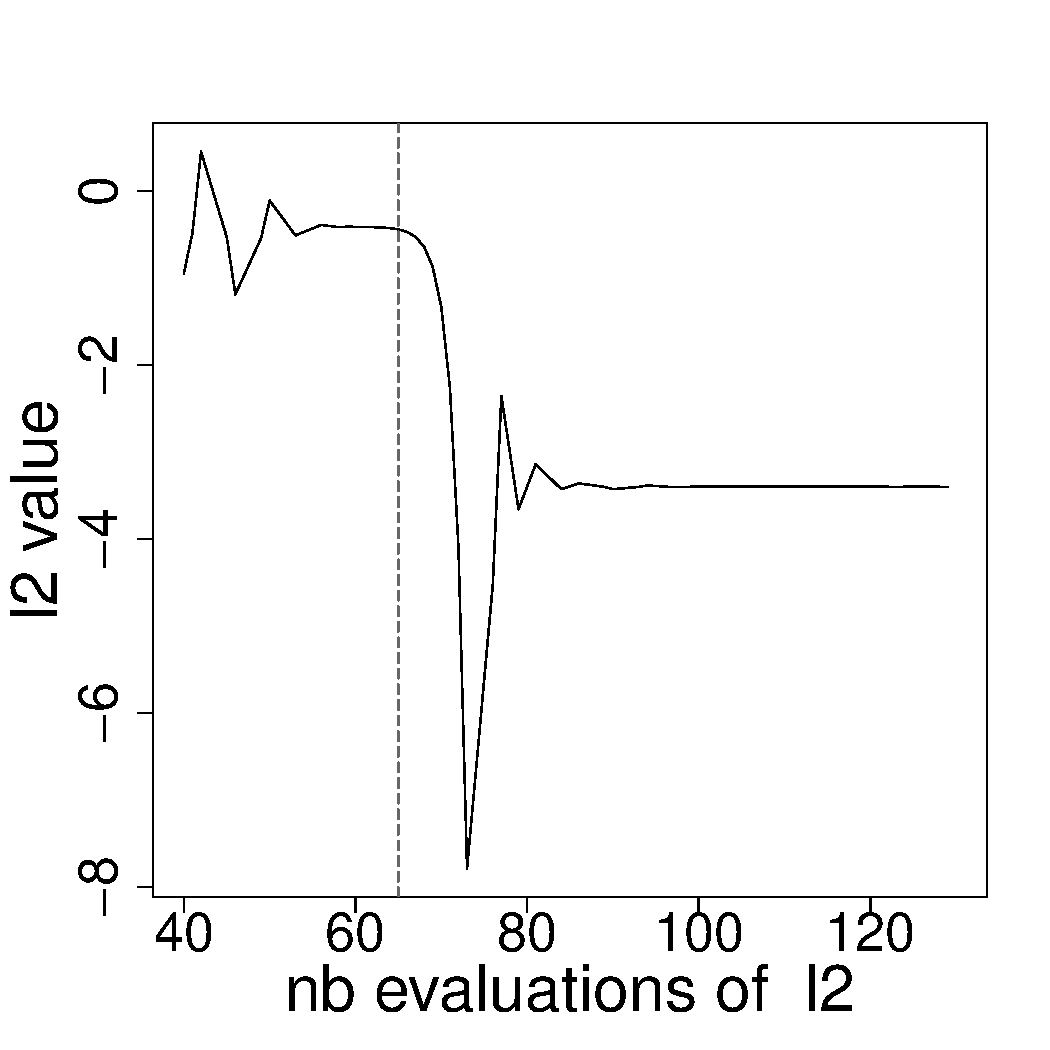
\includegraphics[width=\textwidth]{./R_figs/generated/l2_pertubated}
		%\vspace{-20pt}
		\label{alexandrov_res_pert:l2}
	\end{subfigure}
	\vspace{-20pt}
	\\
	\begin{subfigure}[b]{0.4\textwidth}
		\centering
		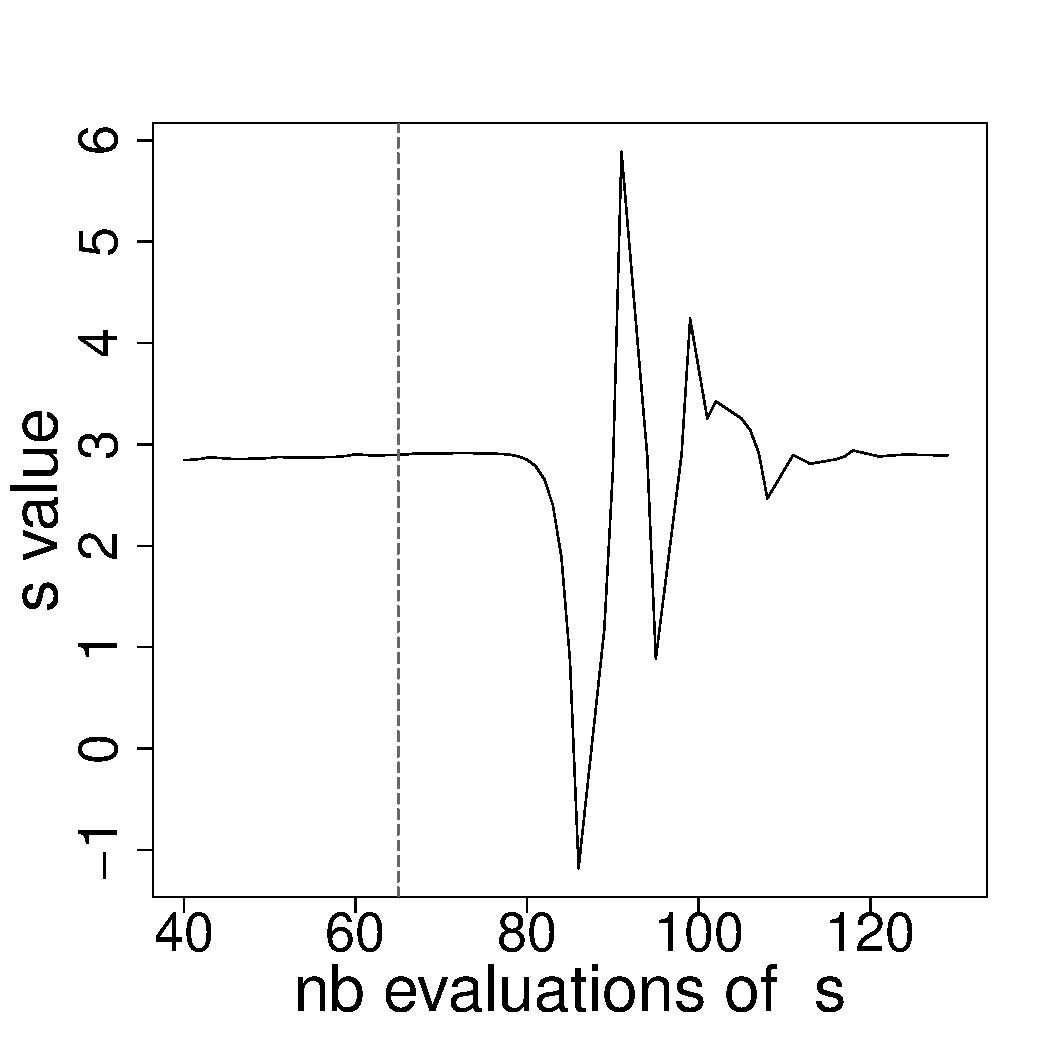
\includegraphics[width=\textwidth]{./R_figs/generated/s_pertubated}
		%\vspace{-20pt}
		\label{alexandrov_res_pert:s}
	\end{subfigure}
	\begin{subfigure}[b]{0.4\textwidth}
		\centering
		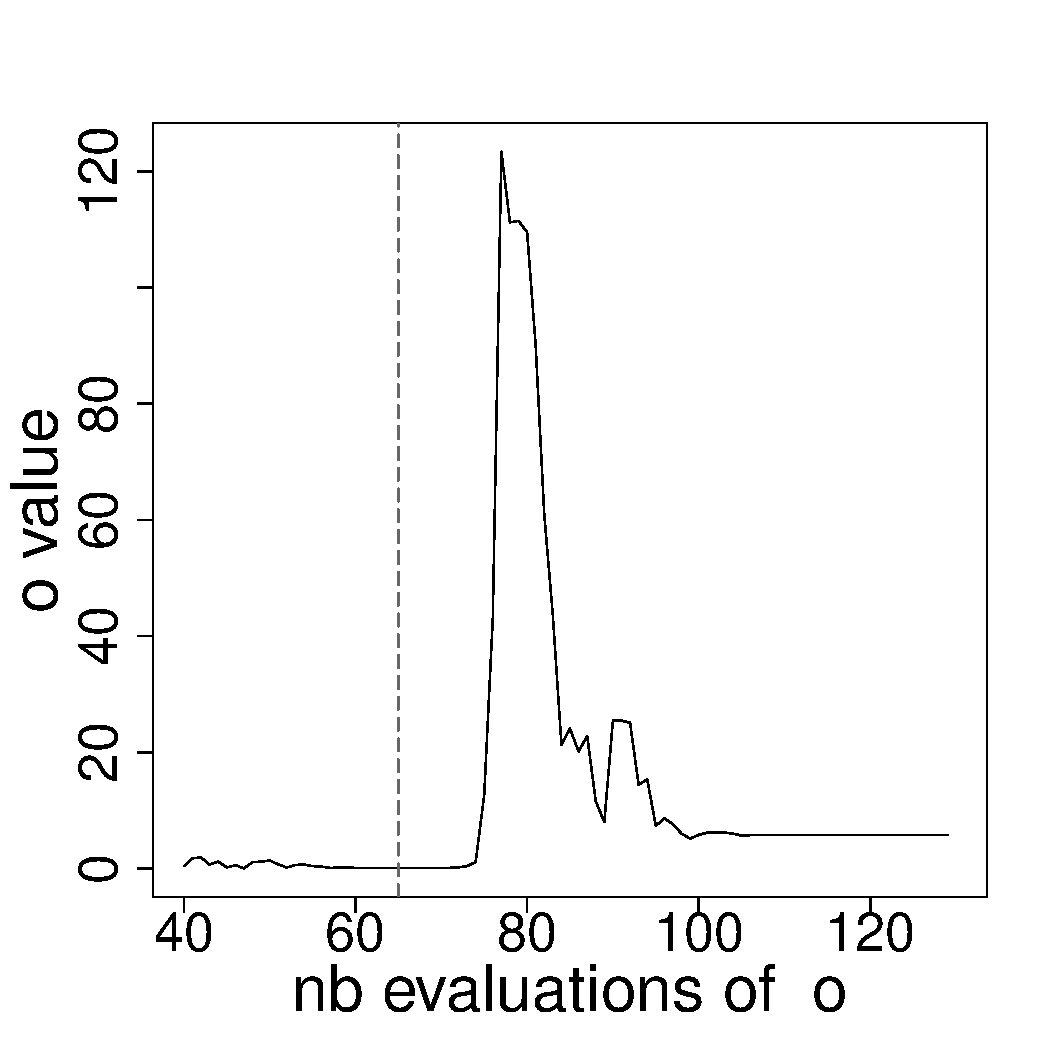
\includegraphics[width=\textwidth]{./R_figs/generated/o_pertubated}
		%\vspace{-20pt}
		\label{alexandrov_res_pert:o}
	\end{subfigure}
	
	\caption{Alexandrov agents behavior with perturbation (constraint change at dotted line)}
	\label{alexandrov_res_pert}
	
\end{figure}

\subsection{Turbofan Problem.}

\begin{figure*}
\centering

  \subfloat{\begin{minipage}{0.27\textwidth}%
		\centering
		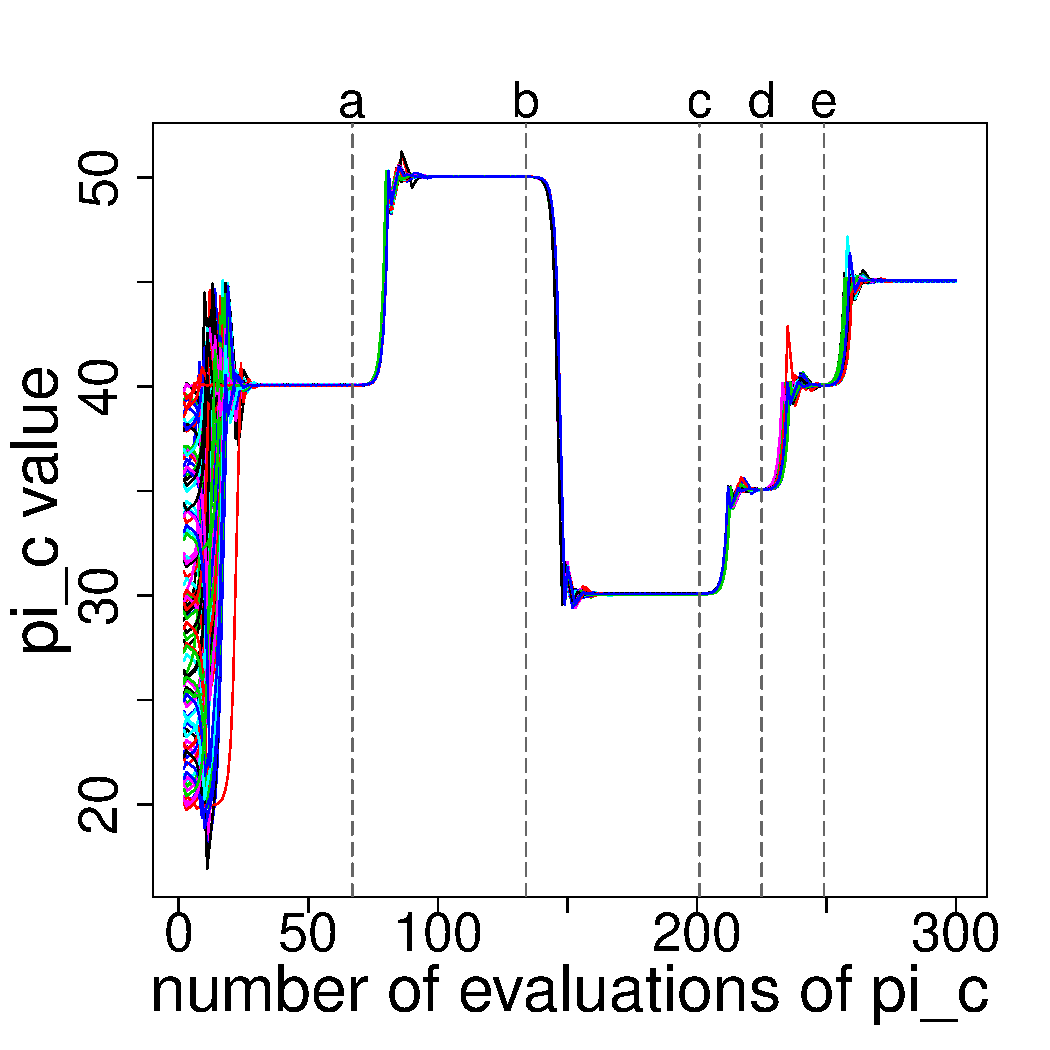
\includegraphics[width=\textwidth]{./R_figs/generated/turbofan_perturbated_pi_c}
		\label{turbofan_res_pert:pi_c}
	\end{minipage}}
	%
	\subfloat{\begin{minipage}{0.27\textwidth}%
		\centering
		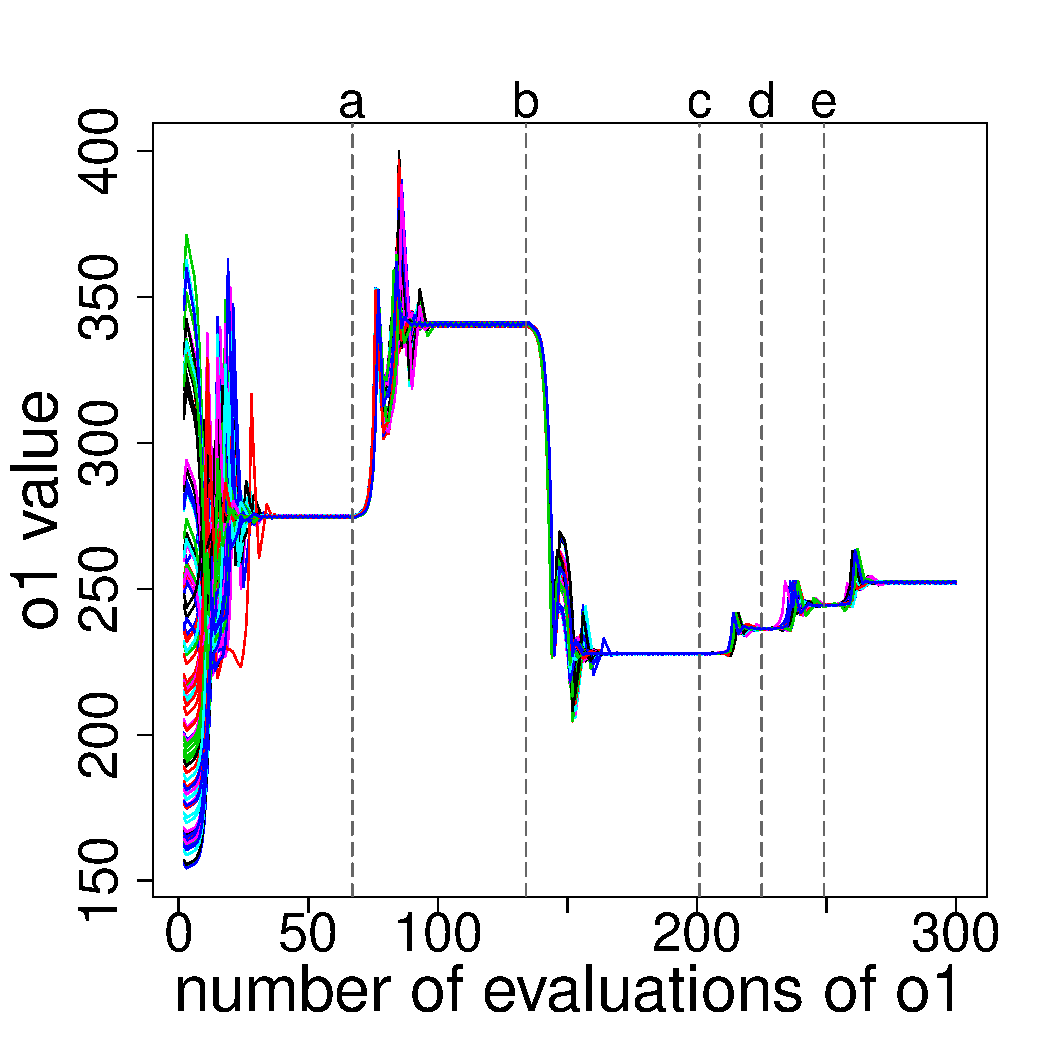
\includegraphics[width=\textwidth]{./R_figs/generated/turbofan_perturbated_o1}
		\label{turbofan_res_pert:o1}
	\end{minipage}}
	%
	\subfloat{\begin{minipage}{0.27\textwidth}%
		\centering
		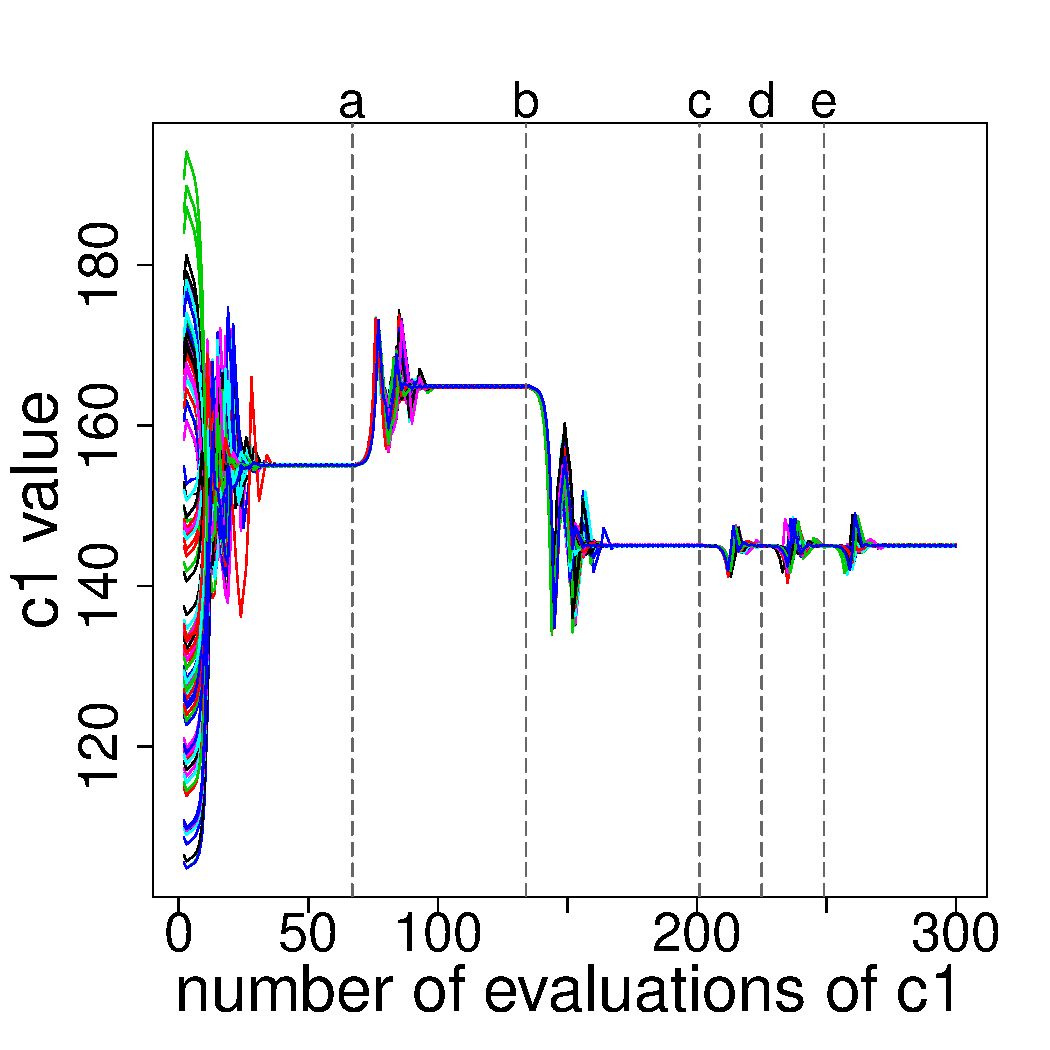
\includegraphics[width=\textwidth]{./R_figs/generated/turbofan_perturbated_c1}
		\label{turbofan_res_pert:c1}
	\end{minipage}}
	%
	\vspace{-20pt}
	\\
	%
	\subfloat{\begin{minipage}{0.27\textwidth}%
		\centering
		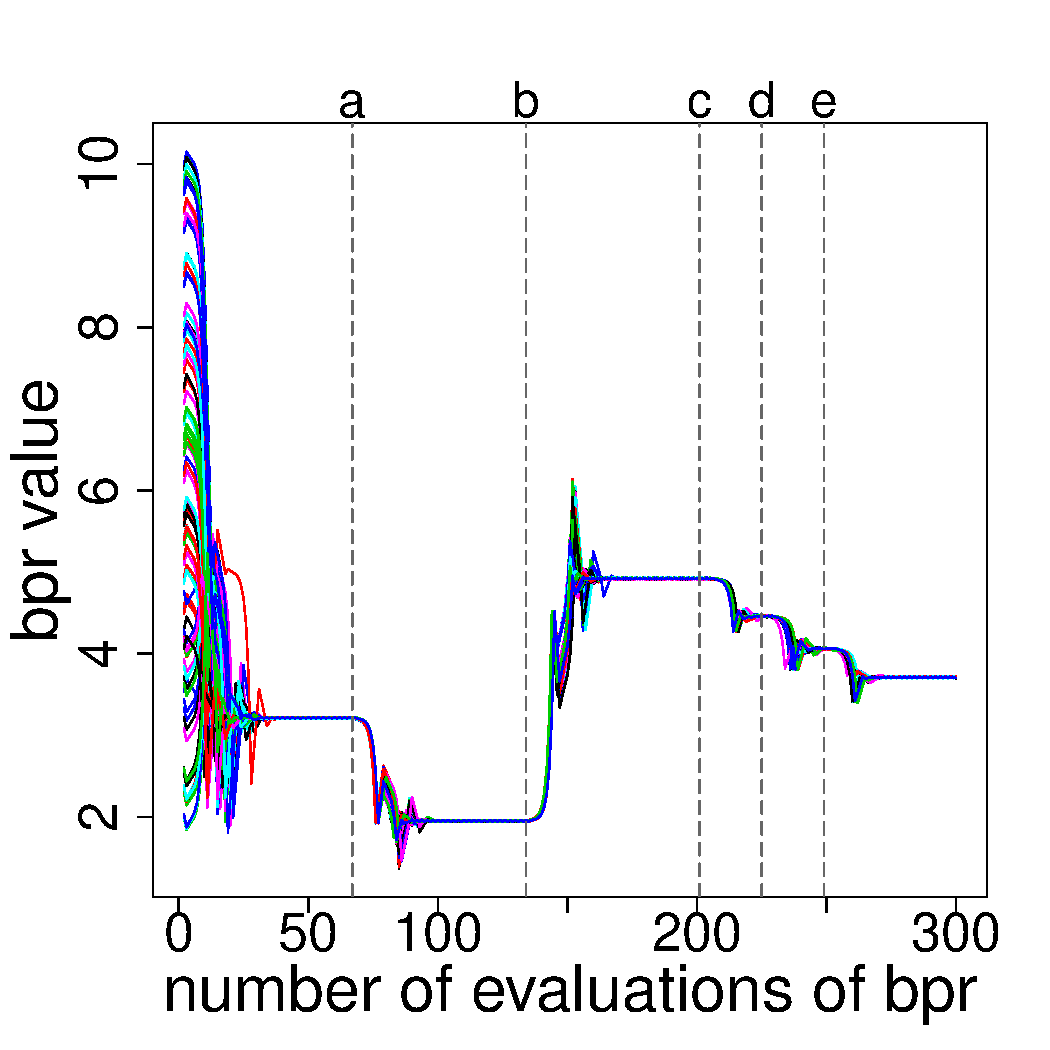
\includegraphics[width=\textwidth]{./R_figs/generated/turbofan_perturbated_bpr}
		\label{turbofan_res_pert:bpr}
	\end{minipage}}
	%	
	\subfloat{\begin{minipage}{0.27\textwidth}%
		\centering
		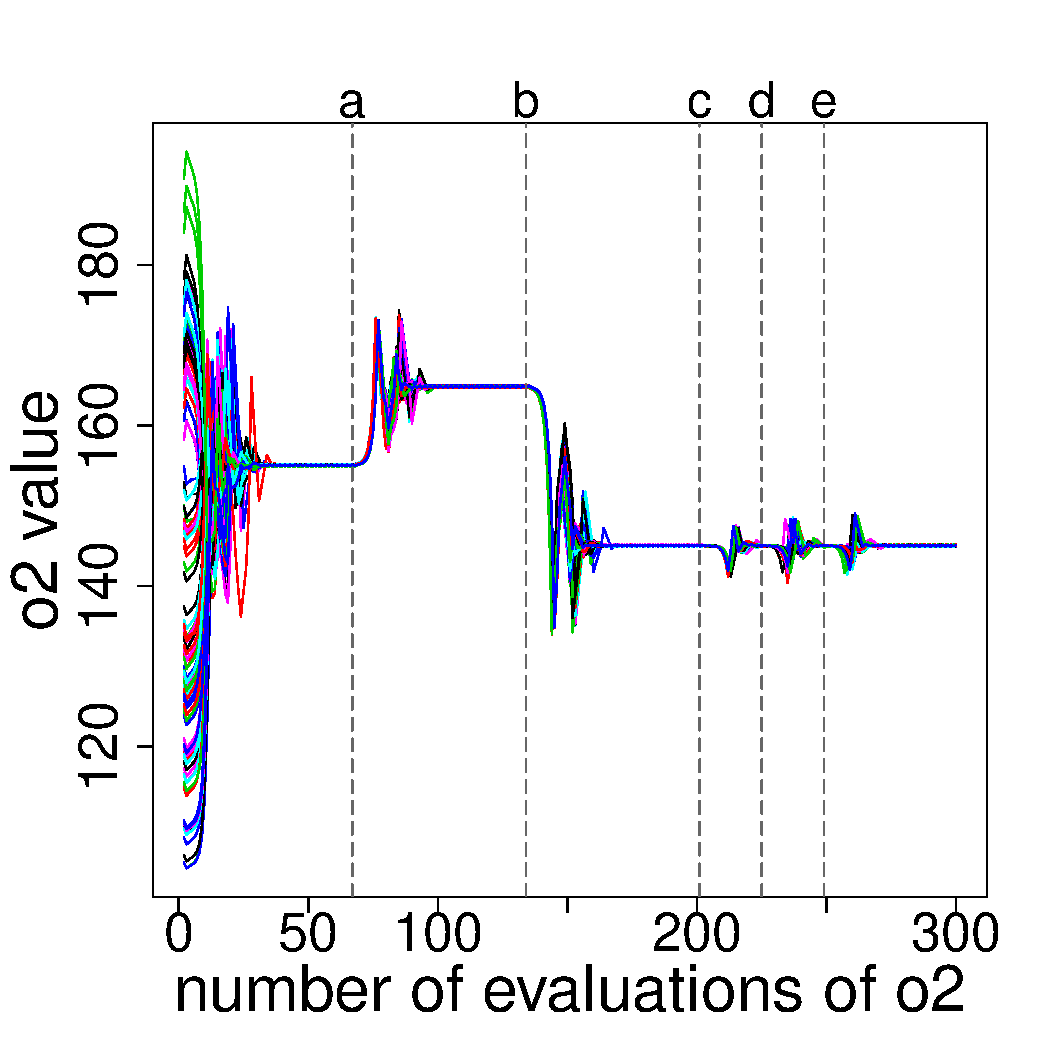
\includegraphics[width=\textwidth]{./R_figs/generated/turbofan_perturbated_o2}
		\label{turbofan_res_pert:o2}
	\end{minipage}}
		%
	\subfloat{\begin{minipage}{0.27\textwidth}%
		\centering
		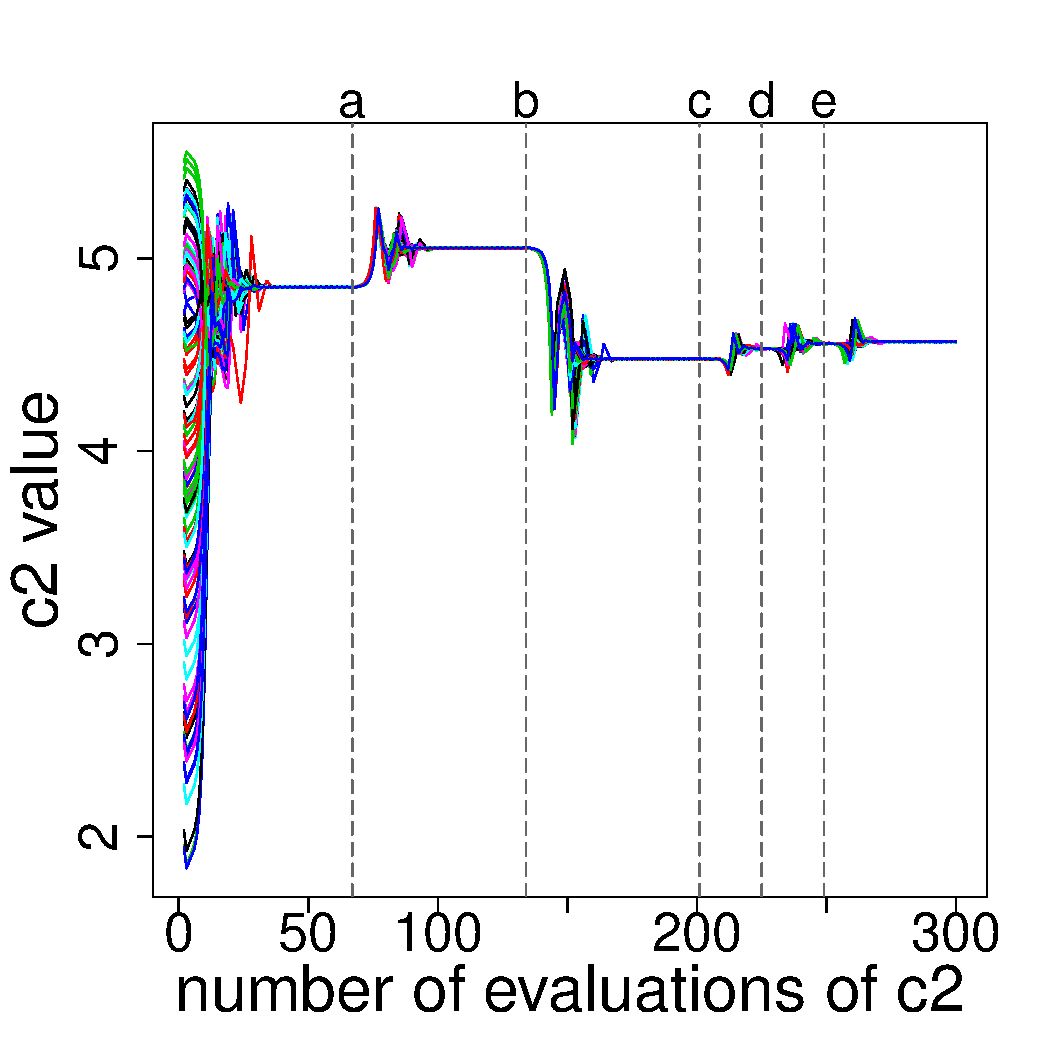
\includegraphics[width=\textwidth]{./R_figs/generated/turbofan_perturbated_c2}
		\label{turbofan_res_pert:c2}
	\end{minipage}}
	
	\caption{Turbofan agents behavior with perturbations (changes at dotted lines)}
	\label{turbofan_res_pert}
\end{figure*}


On \figurename{} \ref{turbofan_res_pert}, we illustrate the adaptation capabilities of the system by subjecting turbofan problem we introduced previously to a series of both strong and faster successive small changes to the problem topology (each perturbation is indicated  by a dotted line). \\
First we create strong changes by modifying simultaneously both a constraint and the definition domain of $pi\_c$:
\begin{description}
\item[a.] $c1$ changed from $s <= 155$ to $s <= 165$, max bound of $pi\_c$ changed from 40 to 50
\item[b.] $c1$ changed from $s <= 165$ to $s <= 145$, max bound of $pi\_c$ changed from 50 to 30
\end{description}
 Then milder perturbations by only changing the definition domain of the variable:
\begin{description}
\item[c.] max bound of $pi\_c$ changed from 30 to 35
\item[d.] max bound of $pi\_c$ changed from 35 to 40
\item[e.] max bound of $pi\_c$ changed from 40 to 45
\end{description}
The experiments show that the system consistently reacts to these perturbations by adapting itself in order to find a new solution for the modified problem.

\subsection{Analysis of Adaptation Capabilities.}

The experiments presented in this section illustrate an interesting property of our MAS. Despite the fact that we never explicitly defined specific behavior rules for the agents to handle dynamics changes, the system is able to dynamically take them in account and adapt to find new satisfactory solutions.

This self-adaptive capability can be explained by two factors. First of all the agents had to be designed considering that previous information they receive can become outdated, as the different parts of the optimization problem do not necessarily converge at the same rate. To this first observation is added the fact that each agent has to keep its reasoning to a local level, since an agent trying to reason on a global level would eventually be overwhelmed by the complexity of the problem. 

The consequence of these two factors is that agents indifferently handle changes caused by the "normal" exploration of the search space and changes made to the optimization problem by the designer. Indeed, from the point of view of an agent, a complex problem and a dynamically changing problem are indistinguishable, and mechanisms tailored to handle one will also help solving the other.

By forcing ourselves to keep the agent behavior at a local level, we gained another advantage in addition of the scalability properties of the MAS. Complex optimization problems requires the agent reasoning to be kept at a local level, both in space (neighborhood and information perceived by the agents) and in time (memorization of the informations). In these conditions, the agent is then \enquote{naturally} able to take in account external changes, are they are not distinguishable from its point of view of \enquote{normal} changes occurring from the optimization process. This characteristic which could at first sight be perceived as a handicap for the agent is in fact a bearer of several benefits.